% =====================================================================
% Rapport généré par scripts/build_latex.py — ne pas éditer à la main.
% Les quatre macros ci-dessous contiennent les espaces réservés à
% compléter avant le rendu final.
% =====================================================================
\newcommand{\reportauthor}{[Prénom NOM]}
\newcommand{\reportsupervisor}{[Nom de l'encadrant]}
\newcommand{\reportinstitution}{[Nom de l'université / de l'école]}
\newcommand{\reportyear}{2025 – 2026}

\documentclass[10pt,a4paper]{article}
\usepackage{fontspec}
\usepackage[french]{babel}
\usepackage[a4paper,top=1.8cm,bottom=1.8cm,left=2.3cm,right=2.0cm]{geometry}
\usepackage{graphicx}
\usepackage{longtable,booktabs,array}
\usepackage{float}
\usepackage{enumitem}
\usepackage{xcolor}
\usepackage{titlesec}
\usepackage{fancyhdr}
\usepackage{amsmath}
\usepackage[hidelinks]{hyperref}

\definecolor{tomate}{HTML}{15803D}
\definecolor{ardoise}{HTML}{475569}

\titleformat{\section}{\Large\bfseries\color{tomate}}{\thesection}{0.8em}{}
\titleformat{\subsection}{\large\bfseries\color{ardoise}}{\thesubsection}{0.6em}{}
\titlespacing*{\section}{0pt}{14pt}{6pt}
\titlespacing*{\subsection}{0pt}{10pt}{4pt}
\setlist{itemsep=1pt,topsep=3pt,parsep=0pt,leftmargin=1.3em}
\setlength{\parindent}{0pt}
\setlength{\parskip}{2pt}
\setlength{\emergencystretch}{3em}
\setlength{\tabcolsep}{3pt}
\renewcommand{\arraystretch}{1.05}

\pagestyle{fancy}
\fancyhf{}
\fancyhead[L]{\small\itshape Détection des maladies de la feuille de tomate}
\fancyhead[R]{\small\thepage}
\renewcommand{\headrulewidth}{0.4pt}

\begin{document}

\begin{titlepage}
\centering
{\small Projet universitaire de fin d'études --- Génie informatique\par}
\vspace{2.4cm}
{\LARGE\bfseries Détection et classification des maladies des plantes à partir d'images de feuilles à l'aide des réseaux de neurones convolutifs (CNN) et du Transfer Learning\par}
\vspace{1.2cm}
{\large\itshape Application au cas de la feuille de tomate --- MobileNetV2, TensorFlow/Keras et Flask\par}
\vfill
\begin{tabular}{@{}r@{\hspace{1em}}l@{}}
Réalisé par : & \reportauthor \\[4pt]
Encadré par : & \reportsupervisor \\[4pt]
Établissement : & \reportinstitution \\[4pt]
Année universitaire : & \reportyear \\
\end{tabular}
\vfill
{\small\itshape Projet universitaire de Deep Learning — document généré depuis le dépôt du projet.\par}
\end{titlepage}

\pagenumbering{roman}
\setcounter{tocdepth}{1}
\tableofcontents
\clearpage
\pagenumbering{arabic}

\clearpage

\section{Introduction générale}
\label{sec:1}% Introduction générale

L'agriculture constitue un secteur économique majeur, particulièrement vulnérable aux maladies des cultures. Parmi les espèces les plus cultivées, la tomate occupe une place de premier plan : elle est produite sur tous les continents et représente une source de revenus importante pour de nombreux exploitants. Or, les maladies foliaires de la tomate --- alternariose précoce, mildiou, moisissure des feuilles, entre autres --- peuvent réduire considérablement les rendements et compromettre une récolte entière en quelques jours.

Le diagnostic de ces maladies repose traditionnellement sur l'expertise humaine : l'agriculteur, le technicien ou l'agronome observe les feuilles, identifie des motifs visuels (taches, halos, duvets, nécroses) et en déduit une pathologie probable. Cette démarche se heurte à plusieurs difficultés : elle exige une formation spécifique, elle est chronophage, elle dépend de la disponibilité d'un expert et elle reste subjective lorsque les symptômes sont discrets ou se ressemblent. De plus, un diagnostic tardif réduit fortement l'efficacité des mesures de protection.

Les progrès récents de l'apprentissage profond (\emph{Deep Learning}) et, en particulier, des réseaux de neurones convolutifs (\emph{Convolutional Neural Networks}, CNN) offrent une alternative prometteuse. Ces modèles sont capables d'apprendre automatiquement des représentations visuelles discriminantes à partir d'exemples étiquetés, sans que l'on ait à définir manuellement les caractéristiques pertinentes. Appliqués à des photographies de feuilles, ils peuvent distinguer une feuille saine d'une feuille malade, et identifier la maladie en cause avec une précision souvent élevée sur des jeux de données de référence.

Le présent projet s'inscrit dans cette dynamique. Il propose un système complet, \textbf{de la donnée brute à l'application Web}, permettant à un utilisateur de téléverser une photographie de feuille de tomate et d'obtenir une prédiction parmi quatre classes, accompagnée d'un score de confiance et de la distribution des probabilités. La démarche s'appuie sur un modèle \textbf{MobileNetV2} pré-entraîné sur ImageNet, adapté par \textbf{Transfer Learning} à notre problème à quatre classes, puis intégré dans une application \textbf{Flask} minimale, en français : téléversement d'une image, puis classe prédite, confiance et distribution des probabilités.

Le rapport est organisé de la manière suivante. Les sections 2 et 3 exposent le contexte, la problématique et les objectifs. Les sections 4 à 6 présentent le cadre théorique : CNN, architecture MobileNetV2 et Transfer Learning. La section 7 décrit le dataset et son exploration, la section 8 le prétraitement et la Data Augmentation. Les sections 9 et 10 détaillent l'architecture du modèle et le protocole d'entraînement. La section 11 est consacrée à l'application Web. Les sections 12 à 14 présentent et discutent les résultats expérimentaux. La section 15 dresse les limites et les perspectives, la section 16 traite de l'éthique et des impacts du système, la section 17 présente la conclusion. La section 18 rassemble les références.

\section{Contexte et problématique}
\label{sec:2}% Contexte et problématique

\subsection{Contexte agricole et scientifique}

La tomate (\emph{Solanum lycopersicum}) est sensible à de nombreuses maladies foliaires d'origine fongique, oomycète, bactérienne ou virale. Trois d'entre elles dominent largement les préoccupations des producteurs :

\begin{itemize}
\item l'\textbf{alternariose précoce}, causée par \emph{Alternaria solani}, qui se manifeste par des taches brunes concentriques sur les feuilles âgées ;
\item le \textbf{mildiou}, causé par \emph{Phytophthora infestans}, dont la progression rapide en conditions humides peut détruire une parcelle en quelques jours ;
\item la \textbf{moisissure des feuilles}, causée par \emph{Passalora fulva}, fréquente sous serre et caractérisée par un duvet olive sur la face inférieure des feuilles.
\end{itemize}

À ces trois pathologies s'ajoute la classe \guillemotleft{} feuille saine \guillemotright{}, indispensable pour que le système apprenne à ne pas signaler de maladie en l'absence de symptôme.

Sur le plan scientifique, la reconnaissance automatique de maladies des plantes à partir d'images est un domaine actif. Le jeu de données \textbf{PlantVillage}, publié par Hughes et Salathé (2015) puis exploité par Mohanty, Hughes et Salathé (2016), a servi de référence à de nombreux travaux. Ces études ont montré que des CNN entraînés sur des images de feuilles peuvent atteindre des précisions supérieures à 99 \% sur ce jeu de données, tout en soulignant une limite essentielle : les performances chutent lorsque les images proviennent de conditions réelles, différentes de celles du laboratoire.

\subsection{Problématique}

La problématique du projet peut être formulée ainsi :

\begin{quote}\small
\textbf{Peut-on concevoir un système accessible, fonctionnant localement et sans service payant, capable de classer automatiquement une photographie de feuille de tomate parmi quatre catégories (saine, alternariose précoce, mildiou, moisissure des feuilles), avec une précision utile, un temps de réponse de l'ordre de la seconde et une interface compréhensible par un utilisateur non spécialiste ?}
\end{quote}

Cette problématique soulève plusieurs sous-questions techniques :

\begin{enumerate}
\item Comment préparer un jeu de données fiable, équilibré et sans fuite entre entraînement et évaluation ?
\item Quel modèle offre le meilleur compromis entre précision et coût de calcul, sachant que l'application doit fonctionner sur un ordinateur sans GPU ?
\item Comment garantir que le prétraitement appliqué lors de la prédiction soit identique à celui utilisé pendant l'entraînement ?
\item Comment présenter le résultat de manière honnête, en affichant la distribution des probabilités plutôt qu'une classe unique présentée comme une certitude ?
\item Comment intégrer le modèle dans une application Web robuste, sécurisée et maintenable ?
\end{enumerate}

\subsection{Enjeu et portée}

L'enjeu n'est pas de remplacer l'expertise agronomique, mais de fournir un \textbf{outil d'aide à la reconnaissance visuelle}, utilisable sur le terrain comme en formation. Le système doit donc être rapide, compréhensible et explicitement présenté comme expérimental. Cette posture est essentielle : un modèle entraîné sur des images de laboratoire ne peut pas prétendre à un diagnostic fiable sur des photographies de terrain.

\section{Objectifs du projet}
\label{sec:3}% Objectifs du projet

\subsection{Objectif général}

Concevoir, entraîner, évaluer et déployer localement une application Web de détection et de classification des maladies de la feuille de tomate, fondée sur un CNN et le Transfer Learning.

\subsection{Objectifs spécifiques}

\textbf{Sur le plan des données}

\begin{itemize}
\item télécharger et organiser le sous-ensemble tomate du dataset PlantVillage ;
\item vérifier l'intégrité des images et détecter les doublons ;
\item construire un découpage stratifié entraînement / validation / test (70 / 15 / 15) reproductible et sans fuite de données ;
\item documenter précisément la provenance, les effectifs et les limites du dataset.
\end{itemize}

\textbf{Sur le plan de la modélisation}

\begin{itemize}
\item construire un modèle MobileNetV2 pré-entraîné sur ImageNet, adapté à quatre classes ;
\item entraîner la tête de classification en base gelée, puis réaliser un fine-tuning partiel ;
\item mettre en place les mécanismes de régularisation et de suivi (Early Stopping, Model Checkpoint, réduction du learning rate, journalisation) ;
\item sauvegarder le meilleur modèle et l'ensemble de ses hyperparamètres.
\end{itemize}

\textbf{Sur le plan de l'évaluation}

\begin{itemize}
\item calculer accuracy, precision, recall et F1-score sur un ensemble de test indépendant ;
\item produire la matrice de confusion, le rapport de classification et les courbes d'apprentissage ;
\item analyser les erreurs et les confusions entre classes ;
\item discuter les limites du modèle.
\end{itemize}

\textbf{Sur le plan applicatif}

\begin{itemize}
\item développer une application Flask en français, limitée à l'essentiel ;
\item proposer une page unique : téléverser une image, afficher le résultat ;
\item ne conserver ni image ni analyse sur le serveur ;
\item valider les fichiers téléversés et éviter de recharger le modèle à chaque requête ;
\item fournir des tests automatisés et une documentation d'installation.
\end{itemize}

\subsection{Contraintes}

Le projet doit rester réalisable par un étudiant en génie informatique, avec des moyens limités : pas de GPU dédié, pas de service cloud payant, pas d'API externe. Toutes les étapes doivent pouvoir être rejouées localement à partir du code fourni.

\section{État de l'art : Deep Learning et réseaux de neurones convolutifs}
\label{sec:4}% État de l'art : Deep Learning et réseaux de neurones convolutifs

\subsection{Du perceptron aux réseaux profonds}

Un réseau de neurones artificiel est composé de couches de neurones interconnectés. Chaque neurone calcule une combinaison linéaire de ses entrées, à laquelle il applique une fonction d'activation non linéaire. L'empilement de plusieurs couches permet d'apprendre des fonctions de plus en plus abstraites. L'apprentissage consiste à ajuster les poids du réseau afin de minimiser une fonction de perte mesurant l'écart entre les prédictions et les étiquettes réelles, généralement par \textbf{descente de gradient} et \textbf{rétropropagation du gradient} (Rumelhart, Hinton et Williams, 1986).

Les réseaux entièrement connectés appliqués directement à des images se heurteraient à un problème de dimension : une image de 224 $\times$ 224 $\times$ 3 contient plus de 150 000 valeurs, et une première couche de 1 000 neurones nécessiterait plus de 150 millions de poids. Les réseaux convolutifs résolvent ce problème en exploitant la structure spatiale des images.

\subsection{Principes des réseaux convolutifs}

\textbf{La convolution.} Une couche de convolution applique un ensemble de filtres (noyaux) de petite taille sur l'image d'entrée. Chaque filtre produit une carte d'activation qui répond à un motif local : contour, texture, couleur. Un filtre de 3 $\times$ 3 partagé sur toute l'image ne possède que 27 poids, ce qui réduit considérablement le nombre de paramètres tout en introduisant deux propriétés fondamentales :

\begin{itemize}
\item le \textbf{partage des poids} : le même détecteur est appliqué partout dans l'image ;
\item l'\textbf{invariance par translation} : un motif reconnu reste reconnu s'il se déplace.
\end{itemize}

\textbf{Le pooling.} Les couches de \emph{max pooling} réduisent la résolution spatiale en conservant la réponse la plus forte de chaque région. Elles diminuent le coût de calcul et rendent la représentation plus robuste aux petites translations.

\textbf{Les fonctions d'activation.} La fonction ReLU (\texttt{max(0, x)}) est la plus utilisée : elle introduit la non-linéarité nécessaire tout en limitant le problème de disparition du gradient. La couche de sortie utilise une fonction \textbf{softmax}, qui transforme un vecteur de scores en une distribution de probabilités dont la somme vaut 1 :

p\_i = exp(z\_i) / somme\_j exp(z\_j), pour i = 1 à 4.

\textbf{La perte et l'optimisation.} Pour une classification multi-classes, la perte usuelle est l'\textbf{entropie croisée catégorielle}. L'optimiseur Adam (Kingma et Ba, 2015) adapte le pas d'apprentissage de chaque paramètre à partir des moments du gradient, ce qui le rend robuste et rapide à converger, avec peu de réglage manuel.

\subsection{Architectures marquantes}

\begin{center}\small\itshape Tableau 1 --- Architectures convolutives marquantes.\end{center}
{\footnotesize
\begin{longtable}{@{}>{\raggedright\arraybackslash}p{0.22\linewidth}>{\raggedright\arraybackslash}p{0.31\linewidth}>{\raggedright\arraybackslash}p{0.33\linewidth}@{}}
\toprule
\textbf{Architecture} & \textbf{Année} & \textbf{Apport principal} \\
\midrule
\endhead
\bottomrule
\endlastfoot
LeNet-5 & 1998 & Premiers succès de la convolution sur les chiffres manuscrits \\
AlexNet & 2012 & Victoire d'ImageNet ; popularisation de ReLU, dropout et GPU \\
VGG-16/19 & 2014 & Empilement régulier de convolutions 3 $\times$ 3 ; simplicité conceptuelle \\
ResNet & 2015 & Connexions résiduelles permettant d'entraîner des réseaux très profonds \\
Inception & 2014 & Convolutions multi-échelles parallèles \\
MobileNet (V1/V2) & 2017-2018 & Convolutions séparables en profondeur, pour les appareils à faibles ressources \\
\end{longtable}
}

Notre choix s'est porté sur MobileNetV2, pour des raisons de coût de calcul et de pertinence pratique : l'application doit fonctionner sur un ordinateur portable sans GPU et produire une prédiction en moins d'une seconde.

\subsection{Régularisation et prévention du sur-apprentissage}

Le sur-apprentissage (\emph{overfitting}) désigne la situation où le modèle mémorise les exemples d'entraînement sans généraliser. Plusieurs techniques sont utilisées dans ce projet :

\begin{itemize}
\item \textbf{Data Augmentation} : création de variantes artificielles des images d'entraînement ;
\item \textbf{Dropout} : désactivation aléatoire de neurones pendant l'entraînement ;
\item \textbf{Early Stopping} : arrêt de l'entraînement lorsque la perte de validation cesse de s'améliorer ;
\item \textbf{réduction du learning rate} : diminution du pas lorsque la validation stagne ;
\item \textbf{poids de classes} : compensation du déséquilibre entre classes ;
\item \textbf{gel des couches pré-entraînées} : limite le nombre de paramètres à apprendre.
\end{itemize}

\subsection{Métriques d'évaluation}

Soit TP, FP, FN et TN les nombres de vrais positifs, faux positifs, faux négatifs et vrais négatifs pour une classe donnée :

\begin{itemize}
\item \textbf{Accuracy} : proportion de prédictions correctes, toutes classes confondues ;
\item \textbf{Precision} : TP / (TP + FP), capacité à ne pas signaler une classe à tort ;
\item \textbf{Recall} : TP / (TP + FN), capacité à retrouver tous les cas de la classe ;
\item \textbf{F1-score} : moyenne harmonique de la precision et du recall.
\end{itemize}

L'accuracy seule est insuffisante en cas de déséquilibre : un modèle qui prédirait toujours la classe majoritaire obtiendrait une accuracy trompeuse. C'est pourquoi la matrice de confusion et les métriques par classe sont systématiquement analysées.

\section{Présentation de MobileNetV2}
\label{sec:5}% Présentation de MobileNetV2

\subsection{Motivation : l'efficacité computationnelle}

MobileNetV2, proposé par Sandler et al. (2018), est une évolution de MobileNet (Howard et al., 2017). Son objectif est de fournir un réseau convolutif performant avec un coût de calcul et un nombre de paramètres très inférieurs à ceux de VGG ou ResNet, afin de permettre une exécution sur téléphone ou micro-ordinateur. Notre modèle complet ne compte ainsi que \textbf{2 422 468 paramètres}, dont seulement \textbf{164 484} sont entraînés lors de la première phase.

\subsection{Convolutions séparables en profondeur}

Une convolution standard de \texttt{Dk $\times$ Dk} noyaux appliquée à \texttt{M} canaux d'entrée pour produire \texttt{N} canaux coûte \texttt{Dk\textsuperscript{2} $\times$ M $\times$ N} multiplications par position. MobileNet la remplace par deux opérations :

\begin{enumerate}
\item une \textbf{convolution en profondeur} (\emph{depthwise}) : un filtre par canal d'entrée, coût \texttt{Dk\textsuperscript{2} $\times$ M} ;
\item une \textbf{convolution ponctuelle} (\emph{pointwise}) 1 $\times$ 1 qui recombine les canaux, coût \texttt{M $\times$ N}.
\end{enumerate}

Le rapport de coût est approximativement \texttt{1/\allowbreak{}N + 1/\allowbreak{}Dk\textsuperscript{2}}, soit une réduction d'environ 8 à 9 fois pour des noyaux 3 $\times$ 3. C'est cette économie qui rend le modèle compatible avec une exécution sur processeur.

\subsection{Blocs résiduels inversés et goulot linéaire}

MobileNetV2 introduit deux idées structurelles :

\begin{itemize}
\item le \textbf{bloc résiduel inversé} (\emph{inverted residual}) : contrairement à ResNet, la connexion résiduelle relie des représentations de faible dimension, tandis que la couche intermédiaire est élargie (facteur d'expansion 6) ;
\item le \textbf{goulot linéaire} (\emph{linear bottleneck}) : la dernière convolution 1 $\times$ 1 de chaque bloc n'applique pas de ReLU, car une activation non linéaire détruirait l'information dans un espace de faible dimension.
\end{itemize}

Le réseau alterne ainsi des blocs d'expansion, de convolution en profondeur et de projection, pour un total de 53 couches convolutives dans la version 1.0 de largeur 224.

\subsection{Sortie et adaptation à notre problème}

La version utilisée est \texttt{MobileNetV2(weights="imagenet", include\_\allowbreak{}top=False)}, avec une entrée de 224 $\times$ 224 $\times$ 3. La couche de classification d'origine (1 000 classes ImageNet) est supprimée. La sortie de la base est un tenseur de forme 7 $\times$ 7 $\times$ 1 280, que nous agrégeons par un \emph{Global Average Pooling} pour obtenir un vecteur de 1 280 caractéristiques. Ce vecteur alimente ensuite notre propre tête de classification.

\subsection{Pourquoi ce choix pour notre projet}

\begin{itemize}
\item \textbf{coût maîtrisé} : entraînement et inférence possibles sur CPU ;
\item \textbf{taille raisonnable} : un fichier modèle de quelques dizaines de mégaoctets ;
\item \textbf{qualité des caractéristiques ImageNet} : textures, contours et couleurs déjà apprises, très utiles pour analyser des feuilles ;
\item \textbf{latence faible} : environ 70 ms par image mesurés sur notre environnement de test.
\end{itemize}

\section{Présentation du Transfer Learning}
\label{sec:6}% Présentation du Transfer Learning

\subsection{Principe}

Le Transfer Learning consiste à réutiliser un modèle entraîné sur une tâche source (généralement ImageNet, 1,2 million d'images et 1 000 classes) pour résoudre une tâche cible disposant de moins de données. Les premières couches d'un CNN apprennent des motifs génériques (contours, couleurs, textures) qui restent pertinents pour de nombreuses tâches visuelles. Seules les couches les plus profondes, spécialisées dans les classes d'origine, doivent être remplacées.

Cette approche est particulièrement adaptée ici : notre dataset ne contient que 5 452 images, un volume insuffisant pour entraîner un CNN profond from scratch sans sur-apprentissage sévère.

\subsection{Deux stratégies complémentaires}

\textbf{Extraction de caractéristiques (feature extraction).} La base pré-entraînée est gelée (\texttt{trainable = False}). Seule la nouvelle tête de classification est entraînée. Le nombre de paramètres apprenables est faible (164 484 dans notre cas), l'entraînement est rapide et le risque de sur-apprentissage limité.

\textbf{Fine-Tuning.} Les dernières couches de la base sont dégelées et ré-entraînées avec un learning rate très faible (1e-5 dans notre cas), afin d'adapter les filtres les plus spécifiques aux textures et couleurs de nos feuilles. Un learning rate élevé détruirait les poids pré-entraînés : c'est pourquoi il doit rester au moins dix fois plus petit que celui de la phase 1.

Dans notre projet, les couches \textbf{BatchNormalization} restent gelées pendant le fine-tuning. Leur mise à jour avec de petits lots (batch de 32) déstabilise l'apprentissage, car les statistiques de normalisation sont estimées sur trop peu d'exemples.

\subsection{Avantages et limites}

\begin{center}\small\itshape Tableau 2 --- Avantages et limites du Transfer Learning.\end{center}
{\footnotesize
\begin{longtable}{@{}>{\raggedright\arraybackslash}p{0.28\linewidth}>{\raggedright\arraybackslash}p{0.58\linewidth}@{}}
\toprule
\textbf{Avantages} & \textbf{Limites} \\
\midrule
\endhead
\bottomrule
\endlastfoot
Apprentissage rapide avec peu de données & Dépend de la similarité entre domaine source et cible \\
Meilleure généralisation qu'un modèle from scratch & Risque de biais hérité d'ImageNet \\
Coût de calcul réduit & Fine-tuning délicat (learning rate, couches à dégeler) \\
Base solide pour un projet étudiant & Ne compense pas un dataset trop pauvre ou mal étiqueté \\
\end{longtable}
}

Le Transfer Learning est donc un levier méthodologique, pas une garantie de performance : la qualité des données et la rigueur de l'évaluation restent déterminantes.

\section{Présentation et exploration du dataset}
\label{sec:7}% Présentation et exploration du dataset

\subsection{Origine des données}

Le dataset utilisé est \textbf{PlantVillage}, un dépôt public d'images de feuilles de plantes saines et malades. Il a été introduit par Hughes et Salathé (2015) et constitue la référence de nombreux travaux en vision par ordinateur appliquée à l'agriculture.

\begin{itemize}
\item \textbf{Source} : dépôt GitHub officiel \texttt{spMohanty/\allowbreak{}PlantVillage-Dataset}, dossier \texttt{raw/\allowbreak{}color} (images couleur d'origine, 256 $\times$ 256 pixels) ;
\item \textbf{Article associé} : Mohanty, Hughes et Salathé (2016), \emph{Using Deep Learning for Image-Based Plant Disease Detection}, Frontiers in Plant Science, 7:1419 ;
\item \textbf{Périmètre retenu} : 4 classes de tomate, soit \textbf{5 452 images}.
\end{itemize}

Le dépôt officiel ne comporte pas de fichier de licence explicite. Les images sont diffusées à des fins de recherche ; elles ont donc été utilisées dans un cadre strictement académique et \textbf{ne sont pas redistribuées} dans le dépôt du projet. Le script \texttt{training/\allowbreak{}download\_\allowbreak{}dataset.py} permet à quiconque de les récupérer depuis la source d'origine.

\subsection{Classes et effectifs}

\begin{center}\small\itshape Tableau 3 --- Classes retenues et effectifs du dataset.\end{center}
{\footnotesize
\begin{longtable}{@{}>{\raggedright\arraybackslash}p{0.24\linewidth}>{\raggedright\arraybackslash}p{0.13\linewidth}>{\raggedright\arraybackslash}p{0.27\linewidth}>{\raggedright\arraybackslash}p{0.22\linewidth}@{}}
\toprule
\textbf{Code de classe} & \textbf{Nom français} & \textbf{Agent pathogène} & \textbf{Images} \\
\midrule
\endhead
\bottomrule
\endlastfoot
\texttt{Tomato\_\allowbreak{}\_\allowbreak{}\_\allowbreak{}Early\_\allowbreak{}blight} & Alternariose précoce & \emph{Alternaria solani} (champignon) & 1 000 \\
\texttt{Tomato\_\allowbreak{}\_\allowbreak{}\_\allowbreak{}Late\_\allowbreak{}blight} & Mildiou de la tomate & \emph{Phytophthora infestans} (oomycète) & 1 909 \\
\texttt{Tomato\_\allowbreak{}\_\allowbreak{}\_\allowbreak{}Leaf\_\allowbreak{}Mold} & Moisissure des feuilles & \emph{Passalora fulva} (champignon) & 952 \\
\texttt{Tomato\_\allowbreak{}\_\allowbreak{}\_\allowbreak{}healthy} & Feuille saine & --- & 1 591 \\
\textbf{Total} &  &  & \textbf{5 452} \\
\end{longtable}
}

Le dataset est \textbf{déséquilibré} : la classe la plus représentée (mildiou, 1 909 images) contient deux fois plus d'images que la classe la moins représentée (moisissure, 952 images). Ce déséquilibre doit être pris en compte, sous peine d'obtenir un modèle qui prédit plus volontiers les classes majoritaires.

\begin{figure}[H]
\centering
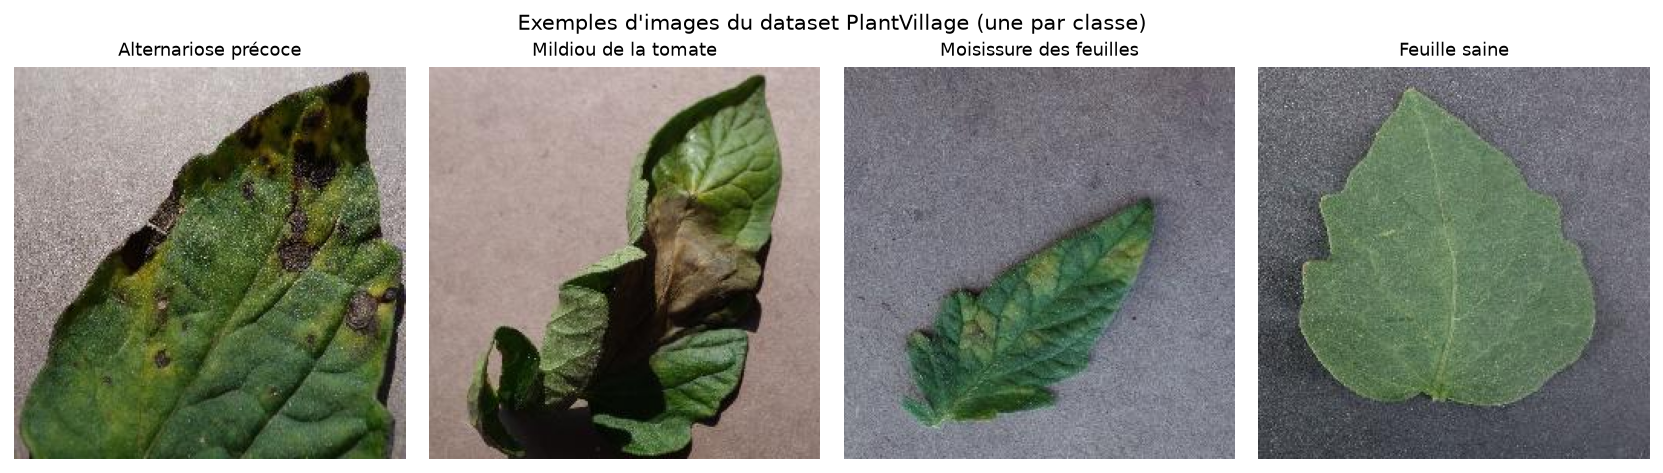
\includegraphics[width=0.68\linewidth,height=0.42\textheight,keepaspectratio]{../../../results/figures/dataset_examples.png}
\par\smallskip{\small\itshape Figure 1 --- Exemples d'images du dataset (une par classe).}
\end{figure}

\subsection{Contrôle qualité}

Avant toute utilisation, chaque fichier a été vérifié :

\begin{itemize}
\item ouverture et décodage complet par Pillow : \textbf{0 image illisible} sur 5 452 ;
\item vérification des dimensions : toutes les images sont en 256 $\times$ 256 pixels, en RGB ;
\item calcul d'une empreinte \textbf{MD5} pour chaque fichier : \textbf{14 doublons exacts} ont été détectés (même image présente plusieurs fois dans le dataset).
\end{itemize}

Les doublons détectés ne sont pas supprimés, car ils correspondent à des images légitimement présentes dans leur classe. En revanche, ils sont \textbf{regroupés} lors du découpage afin qu'une même image ne puisse jamais se retrouver simultanément dans l'ensemble d'entraînement et dans l'ensemble de test.

\subsection{Découpage des données}

Le découpage est réalisé par classe (stratifié), avec la graine aléatoire \textbf{42} pour garantir la reproductibilité, selon les proportions 70 \% / 15 \% / 15 \% :

\begin{center}\small\itshape Tableau 4 --- Rôle et taille des trois ensembles.\end{center}
{\footnotesize
\begin{longtable}{@{}>{\raggedright\arraybackslash}p{0.22\linewidth}>{\raggedright\arraybackslash}p{0.31\linewidth}>{\raggedright\arraybackslash}p{0.33\linewidth}@{}}
\toprule
\textbf{Ensemble} & \textbf{Rôle} & \textbf{Images} \\
\midrule
\endhead
\bottomrule
\endlastfoot
Entraînement & Apprentissage des poids & 3 811 \\
Validation & Suivi, Early Stopping, sélection du modèle & 821 \\
Test & Évaluation finale, jamais utilisé pendant l'entraînement & 820 \\
\end{longtable}
}

La répartition détaillée par classe est la suivante :

\begin{center}\small\itshape Tableau 5 --- Découpage stratifié détaillé par classe.\end{center}
{\footnotesize
\begin{longtable}{@{}>{\raggedright\arraybackslash}p{0.24\linewidth}>{\raggedright\arraybackslash}p{0.13\linewidth}>{\raggedright\arraybackslash}p{0.27\linewidth}>{\raggedright\arraybackslash}p{0.22\linewidth}@{}}
\toprule
\textbf{Classe} & \textbf{Entraînement} & \textbf{Validation} & \textbf{Test} \\
\midrule
\endhead
\bottomrule
\endlastfoot
Alternariose précoce & 700 & 150 & 150 \\
Mildiou de la tomate & 1 334 & 288 & 287 \\
Moisissure des feuilles & 666 & 143 & 143 \\
Feuille saine & 1 111 & 240 & 240 \\
\textbf{Total} & \textbf{3 811} & \textbf{821} & \textbf{820} \\
\end{longtable}
}

\begin{figure}[H]
\centering
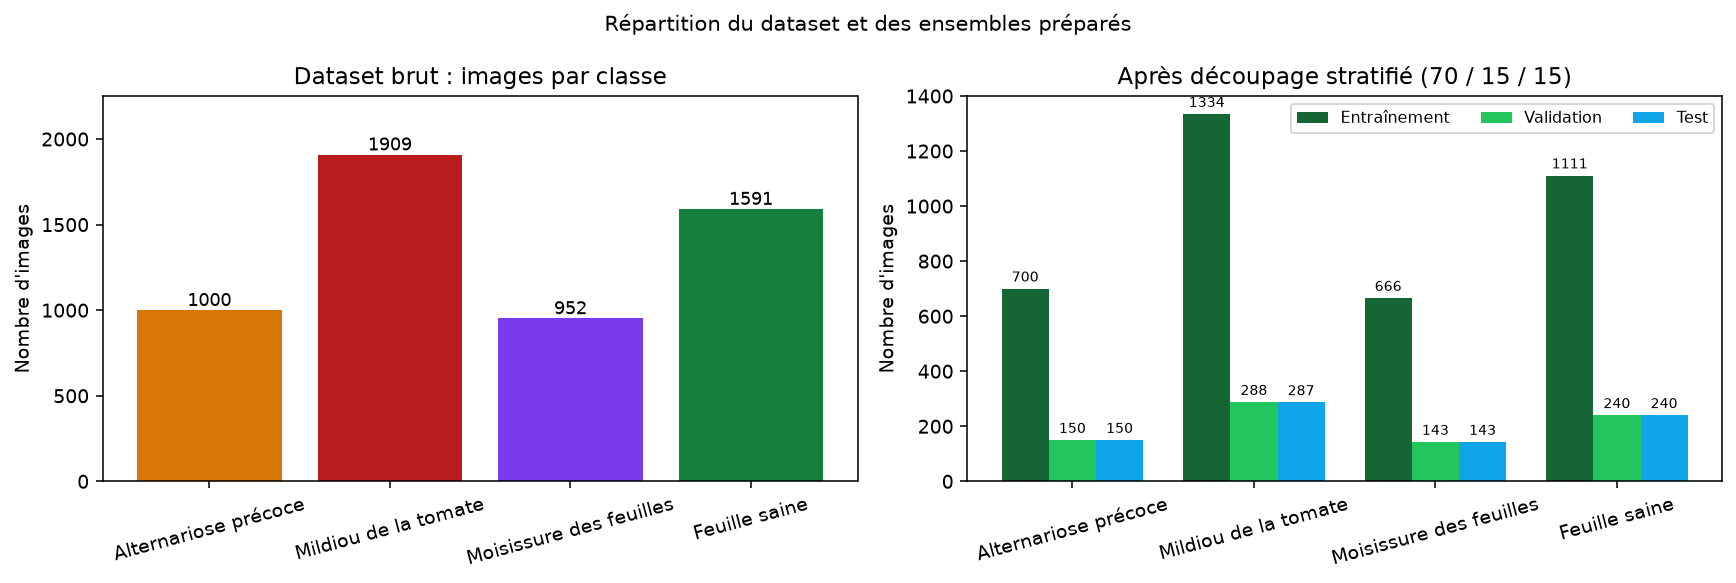
\includegraphics[width=0.68\linewidth,height=0.42\textheight,keepaspectratio]{../../../results/figures/dataset_distribution.png}
\par\smallskip{\small\itshape Figure 2 --- Répartition des images par classe, avant et après découpage.}
\end{figure}

\subsection{Garanties contre la fuite de données}

La fuite de données (\emph{data leakage}) est l'une des erreurs les plus fréquentes en apprentissage automatique : si des images très similaires se trouvent à la fois dans l'entraînement et dans le test, les performances mesurées sont artificiellement optimistes. Trois mesures ont été prises :

\begin{enumerate}
\item \textbf{découpage au niveau des fichiers, avant tout calcul de statistiques} ;
\item \textbf{regroupement des doublons exacts} dans un même ensemble ;
\item \textbf{absence totale d'utilisation du test} pendant l'entraînement et la sélection du modèle (le test n'est chargé que par \texttt{training/\allowbreak{}evaluate.py}).
\end{enumerate}

\subsection{Limites du dataset}

\begin{itemize}
\item \textbf{Images de laboratoire} : les feuilles sont photographiées sur un fond uniforme, souvent gris, avec un éclairage contrôlé. Les performances mesurées ne peuvent pas être transposées directement à des photos prises au champ.
\item \textbf{Une seule culture} : le modèle ne connaît que la tomate.
\item \textbf{Pas de niveau de gravité} : seules les classes sont étiquetées, pas le stade de la maladie.
\item \textbf{Regroupement par feuille} : le dépôt fournit des métadonnées de regroupement par feuille (\emph{leaf grouping}) que nous n'avons pas exploitées ; des images d'une même feuille sous des angles légèrement différents peuvent donc se retrouver dans deux ensembles. C'est une limite reconnue, qui plaide pour une évaluation future plus stricte.
\item \textbf{Quatre classes sur trente-huit} : les autres maladies de la tomate (septoriose, brûlure bactérienne, virus de l'enroulement jaune, tache cible, etc.) sont hors périmètre et seront de toute façon classées dans l'une des quatre catégories.
\end{itemize}

\section{Prétraitement et Data Augmentation}
\label{sec:8}% Prétraitement et Data Augmentation

\subsection{Pipeline de prétraitement}

Le prétraitement est \textbf{strictement identique} pendant l'entraînement et pendant la prédiction. Il est centralisé dans \texttt{utils/\allowbreak{}preprocessing.py}, utilisé à la fois par les scripts d'entraînement et par l'application Flask.

\begin{center}\small\itshape Tableau 6 --- Pipeline de prétraitement des images.\end{center}
{\footnotesize
\begin{longtable}{@{}>{\raggedright\arraybackslash}p{0.22\linewidth}>{\raggedright\arraybackslash}p{0.31\linewidth}>{\raggedright\arraybackslash}p{0.33\linewidth}@{}}
\toprule
\textbf{Étape} & \textbf{Opération} & \textbf{Justification} \\
\midrule
\endhead
\bottomrule
\endlastfoot
1 & Ouverture et conversion en RGB & Uniformise les images (PNG avec transparence, niveaux de gris, etc.) \\
2 & Application de l'orientation EXIF & Corrige les photos de smartphone \\
3 & Redimensionnement en 224 $\times$ 224 & Taille d'entrée attendue par MobileNetV2 \\
4 & Conversion en tableau \texttt{float32} & Format numérique attendu par Keras \\
5 & Normalisation \texttt{x /\allowbreak{} 127.5 - 1} & Ramène les valeurs dans [-1, 1], convention MobileNetV2 \\
\end{longtable}
}

La normalisation utilisée reproduit exactement \texttt{tensorflow.keras.applications.mobilenet\_\allowbreak{}v2.preprocess\_\allowbreak{}input}. Un test automatisé (\texttt{tests/\allowbreak{}test\_\allowbreak{}preprocessing.py}) vérifie cette équivalence numériquement, ce qui garantit l'absence de décalage de distribution entre l'entraînement et l'inférence : c'est un point où de nombreux projets échouent silencieusement.

\subsection{Data Augmentation}

La Data Augmentation génère des variantes des images d'entraînement afin d'augmenter la diversité apparente du dataset et de réduire le sur-apprentissage. Les transformations retenues sont volontairement modérées, car les images PlantVillage sont déjà cadrées et centrées :

\begin{center}\small\itshape Tableau 7 --- Transformations de Data Augmentation.\end{center}
{\footnotesize
\begin{longtable}{@{}>{\raggedright\arraybackslash}p{0.22\linewidth}>{\raggedright\arraybackslash}p{0.31\linewidth}>{\raggedright\arraybackslash}p{0.33\linewidth}@{}}
\toprule
\textbf{Transformation} & \textbf{Paramètre} & \textbf{Effet recherché} \\
\midrule
\endhead
\bottomrule
\endlastfoot
Rotation & $\pm$5 \% ($\approx$ $\pm$18\textdegree{}) & Robustesse à l'orientation de la feuille \\
Zoom & $\pm$10 \% & Robustesse à la distance de prise de vue \\
Retournement horizontal & aléatoire & Invariance gauche/droite \\
Luminosité & $\pm$15 \% & Robustesse aux conditions d'éclairage \\
Translation & $\pm$5 \% & Robustesse au cadrage \\
\end{longtable}
}

Ces couches sont appliquées \textbf{uniquement} au jeu d'entraînement et sont inactives à l'inférence. Elles ne font pas partie du modèle sauvegardé : le prétraitement de prédiction reste donc simplement \guillemotleft{} redimensionnement + normalisation \guillemotright{}.

\begin{figure}[H]
\centering
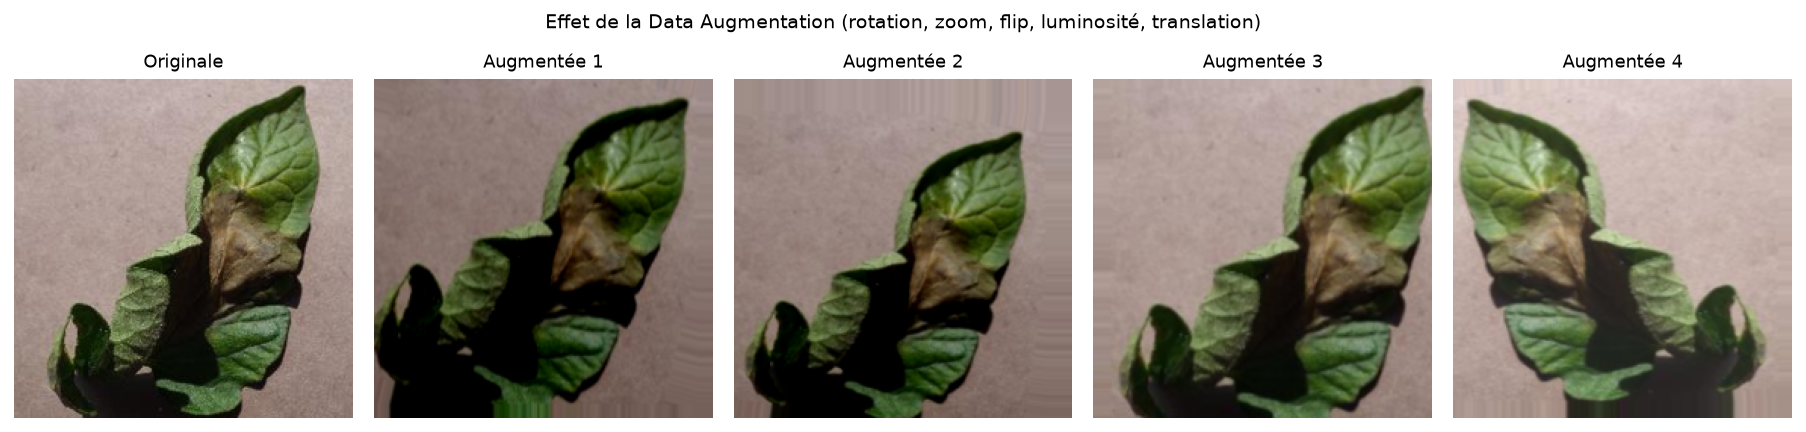
\includegraphics[width=0.68\linewidth,height=0.42\textheight,keepaspectratio]{../../../results/figures/augmentation_examples.png}
\par\smallskip{\small\itshape Figure 3 --- Exemples de variantes générées par la Data Augmentation sur une même image.}
\end{figure}

\subsection{Gestion du déséquilibre des classes}

Deux mécanismes complémentaires ont été mis en place :

\begin{enumerate}
\item \textbf{poids de classes} lors de la phase 1 : chaque classe reçoit un poids inversement proportionnel à son effectif (mildiou $\approx$ 0,72 ; alternariose $\approx$ 1,36 ; moisissure $\approx$ 1,43 ; feuille saine $\approx$ 0,86) ;
\item \textbf{métriques par classe} dans l'évaluation, afin de ne pas masquer une classe défavorisée par une bonne accuracy globale.
\end{enumerate}

\section{Architecture du modèle proposé}
\label{sec:9}% Architecture du modèle proposé

\subsection{Vue d'ensemble}

Le modèle est construit en Keras selon l'enchaînement suivant :

\begin{enumerate}
\item entrée de forme 224 $\times$ 224 $\times$ 3 ;
\item base \textbf{MobileNetV2} pré-entraînée sur ImageNet, sans couche de classification (\texttt{include\_\allowbreak{}top=False}) ;
\item \textbf{GlobalAveragePooling2D} : agrège les 7 $\times$ 7 $\times$ 1 280 cartes en un vecteur de 1 280 ;
\item \textbf{Dropout (0,2)} ;
\item \textbf{Dense(128, activation ReLU)} : couche de caractéristiques spécifiques au problème ;
\item \textbf{Dropout (0,3)} ;
\item \textbf{Dense(4, activation Softmax)} : distribution de probabilités sur les quatre classes.
\end{enumerate}

\begin{figure}[H]
\centering
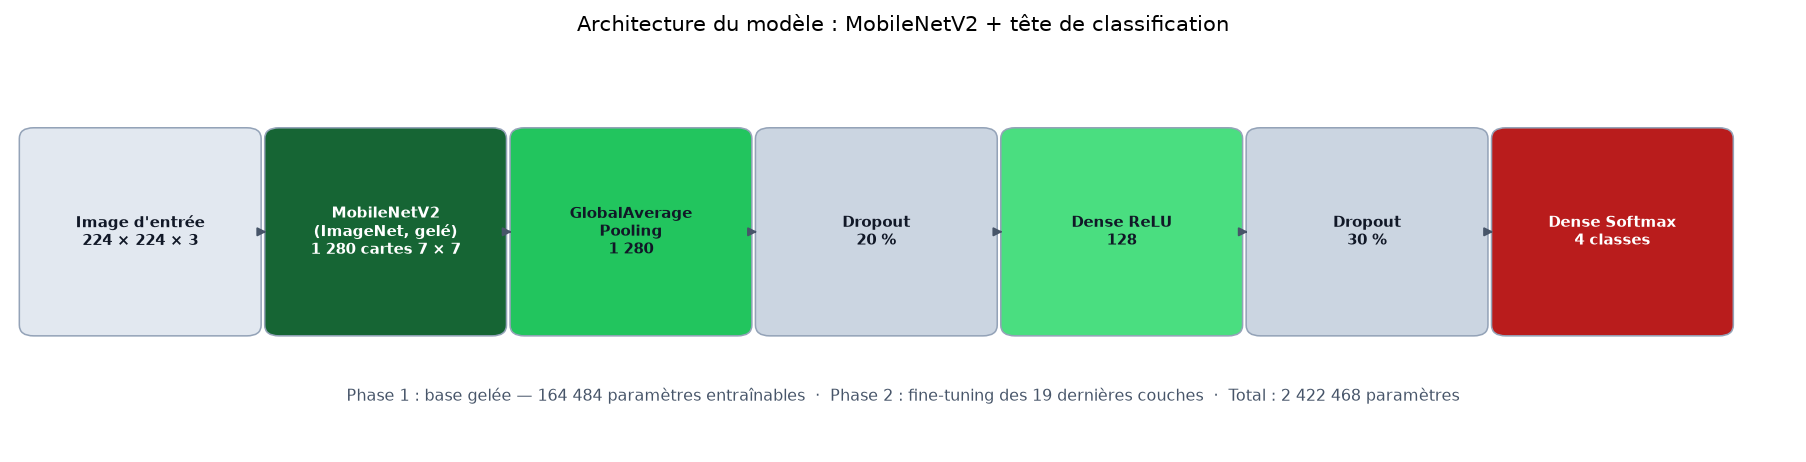
\includegraphics[width=0.68\linewidth,height=0.42\textheight,keepaspectratio]{../../../results/figures/model_architecture.png}
\par\smallskip{\small\itshape Figure 4 --- Architecture du modèle : base MobileNetV2 et tête de classification.}
\end{figure}

\subsection{Détail des couches et des paramètres}

\begin{center}\small\itshape Tableau 8 --- Détail des couches et du nombre de paramètres.\end{center}
{\footnotesize
\begin{longtable}{@{}>{\raggedright\arraybackslash}p{0.24\linewidth}>{\raggedright\arraybackslash}p{0.13\linewidth}>{\raggedright\arraybackslash}p{0.27\linewidth}>{\raggedright\arraybackslash}p{0.22\linewidth}@{}}
\toprule
\textbf{Bloc} & \textbf{Type} & \textbf{Sortie} & \textbf{Paramètres} \\
\midrule
\endhead
\bottomrule
\endlastfoot
Entrée & InputLayer & 224 $\times$ 224 $\times$ 3 & 0 \\
Base & MobileNetV2 (ImageNet) & 7 $\times$ 7 $\times$ 1 280 & 2 257 984 \\
Agrégation & GlobalAveragePooling2D & 1 280 & 0 \\
Régularisation & Dropout (0,2) & 1 280 & 0 \\
Classification & Dense (ReLU) & 128 & 163 968 \\
Régularisation & Dropout (0,3) & 128 & 0 \\
Sortie & Dense (Softmax) & 4 & 516 \\
\textbf{Total} &  &  & \textbf{2 422 468} \\
\end{longtable}
}

Les 2 257 984 paramètres de la base sont \textbf{gelés} en phase 1 : seuls 164 484 paramètres sont alors entraînables, soit moins de 7 \% du total. Cette réduction drastique explique la rapidité de convergence observée.

\subsection{Choix de la fonction de perte et de l'optimiseur}

\begin{itemize}
\item \textbf{Perte} : \texttt{categorical\_\allowbreak{}crossentropy}, adaptée à un encodage one-hot des étiquettes (les images sont chargées avec \texttt{label\_\allowbreak{}mode="categorical"}).
\item \textbf{Optimiseur} : Adam, avec un learning rate de 1e-3 en phase 1 puis 1e-5 en phase 2.
\item \textbf{Métrique suivie} : accuracy, complétée par la perte de validation pour l'Early Stopping et la réduction du learning rate.
\end{itemize}

Le choix d'Adam se justifie par sa robustesse et sa convergence rapide sans réglage fin du pas, ce qui est adapté à un projet où le nombre d'expériences possibles est limité par le temps de calcul.

\section{Configuration et processus d'entraînement}
\label{sec:10}% Configuration et processus d'entraînement

\subsection{Hyperparamètres}

\begin{center}\small\itshape Tableau 9 --- Hyperparamètres d'entraînement.\end{center}
{\footnotesize
\begin{longtable}{@{}>{\raggedright\arraybackslash}p{0.28\linewidth}>{\raggedright\arraybackslash}p{0.58\linewidth}@{}}
\toprule
\textbf{Paramètre} & \textbf{Valeur} \\
\midrule
\endhead
\bottomrule
\endlastfoot
Taille d'image & 224 $\times$ 224 $\times$ 3 \\
Batch size & 32 \\
Époques maximales (phase 1) & 15 (configuration : 30) \\
Époques maximales (phase 2) & 8 (configuration : 15) \\
Learning rate phase 1 & 1e-3 \\
Learning rate phase 2 & 1e-5 \\
Couches dégelées & 19 (30 dernières couches, BatchNormalization exclues) \\
Perte & Categorical crossentropy \\
Optimiseur & Adam \\
Graine aléatoire & 42 \\
Early Stopping & patience 5 sur \texttt{val\_\allowbreak{}loss}, restauration des meilleurs poids \\
Model Checkpoint & sauvegarde si \texttt{val\_\allowbreak{}accuracy} s'améliore \\
ReduceLROnPlateau & facteur 0,5, patience 2, learning rate minimal 1e-6 \\
\end{longtable}
}

\begin{quote}\small
\textbf{Remarque sur le budget d'époques.} Le nombre maximal d'époques prévu par la configuration est de 30 (phase 1) et 15 (phase 2). L'expérience présentée ici a été exécutée avec un budget réduit (15 + 8 époques) car elle a été réalisée sur un processeur à deux cœurs, sans GPU : chaque époque dure environ 90 secondes. Ce budget reste suffisant pour observer la convergence, comme le montrent les courbes.
\end{quote}

\subsection{Environnement d'exécution}

\begin{center}\small\itshape Tableau 10 --- Environnement d'exécution de l'expérience.\end{center}
{\footnotesize
\begin{longtable}{@{}>{\raggedright\arraybackslash}p{0.28\linewidth}>{\raggedright\arraybackslash}p{0.58\linewidth}@{}}
\toprule
\textbf{Élément} & \textbf{Valeur} \\
\midrule
\endhead
\bottomrule
\endlastfoot
Processeur & 2 cœurs (x86-64, AVX2) \\
Mémoire & 16 Go \\
GPU & aucun \\
Système & Linux (Ubuntu 24.04) \\
Python & 3.12 \\
TensorFlow & 2.21 (version CPU) \\
Durée phase 1 & 23,4 minutes (15 époques) \\
Durée phase 2 & 14,3 minutes (8 époques) \\
Durée totale & $\approx$ 38 minutes \\
\end{longtable}
}

\subsection{Déroulement de la phase 1}

La base MobileNetV2 est gelée et seules les couches de classification apprennent. Dès la première époque, l'accuracy de validation atteint \textbf{86,2 \%}, ce qui illustre la qualité des caractéristiques ImageNet. La progression est rapide : 89,40 \% à l'époque 2, 91,84 \% à l'époque 3, puis un maximum de \textbf{94,52 \% dès l'époque 4}. La validation oscille ensuite entre 91 \% et 94,5 \% jusqu'à la fin de la phase. Le learning rate est réduit automatiquement à 5e-4 puis 2,5e-4 et 1,25e-4, sans gain supplémentaire sur la validation : le modèle commence à plafonner.

\subsection{Déroulement de la phase 2 (fine-tuning)}

Les 19 dernières couches de la base sont dégelées et ré-entraînées avec un learning rate de 1e-5. Après une légère dégradation initiale (92,8 \% à l'époque 16), la validation remonte progressivement. Les époques 21 et 22 apportent les meilleurs résultats :

\begin{itemize}
\item époque 18 : 92,81 \% ;
\item époque 20 : 94,76 \% ;
\item époque 21 : 94,52 \% ;
\item \textbf{époque 22 : 95,98 \%} (meilleur modèle retenu) ;
\item époque 23 : 94,52 \% (légère baisse, non conservée).
\end{itemize}

Le fine-tuning apporte donc un gain réel de \textbf{+1,46 point} d'accuracy de validation par rapport au meilleur modèle de la phase 1 (94,52 \% $\rightarrow$ 95,98 \%). Le meilleur modèle est sauvegardé automatiquement dans \texttt{models/\allowbreak{}best\_\allowbreak{}model.keras}, avec la contrainte de ne jamais remplacer un modèle de phase 1 par un modèle de phase 2 moins bon (\texttt{initial\_\allowbreak{}value\_\allowbreak{}threshold}).

\subsection{Suivi et reproductibilité}

Tous les paramètres, comptages, durées et versions de bibliothèques sont enregistrés dans \texttt{models/\allowbreak{}training\_\allowbreak{}config.json}. L'historique complet des époques est conservé dans \texttt{results/\allowbreak{}metrics/\allowbreak{}training\_\allowbreak{}history.json} et \texttt{results/\allowbreak{}metrics/\allowbreak{}training\_\allowbreak{}log.csv}. La graine 42 est fixée pour Python, NumPy et TensorFlow. Le découpage des données est lui aussi déterministe. Ces précautions permettent de rejouer l'expérience dans des conditions comparables.

\section{Développement de l'application Web}
\label{sec:11}% Développement de l'application Web

\subsection{Objectif et principe}

L'application Web constitue la couche de restitution du projet : elle rend le modèle utilisable par une personne qui ne connaît rien à l'apprentissage automatique. Son périmètre a été volontairement limité à \textbf{une seule fonction} : recevoir une image de feuille et afficher la prédiction du modèle.

Deux routes suffisent :

{\footnotesize
\begin{longtable}{@{}>{\raggedright\arraybackslash}p{0.22\linewidth}>{\raggedright\arraybackslash}p{0.31\linewidth}>{\raggedright\arraybackslash}p{0.33\linewidth}@{}}
\toprule
\textbf{Route} & \textbf{Méthode} & \textbf{Rôle} \\
\midrule
\endhead
\bottomrule
\endlastfoot
\texttt{/\allowbreak{}} & GET & affiche le formulaire de téléversement \\
\texttt{/\allowbreak{}analyser} & POST & valide l'image, lance la prédiction, réaffiche la page avec le résultat \\
\end{longtable}
}

Le modèle Keras est chargé \textbf{une seule fois} au démarrage (singleton protégé par un verrou) : chaque analyse évite ainsi plusieurs secondes de chargement. L'application ne maintient ni session, ni compte, ni base de données.

\subsection{Architecture}

Le code reste organisé par responsabilité, comme le reste du projet :

\begin{center}\small\itshape Tableau 11 --- Modules de l'application et responsabilités.\end{center}
{\footnotesize
\begin{longtable}{@{}>{\raggedright\arraybackslash}p{0.28\linewidth}>{\raggedright\arraybackslash}p{0.58\linewidth}@{}}
\toprule
\textbf{Module} & \textbf{Responsabilité} \\
\midrule
\endhead
\bottomrule
\endlastfoot
\texttt{config.py} & chemins, hyperparamètres, libellés français des classes \\
\texttt{app.py} & les deux routes, la validation, le rendu de la page \\
\texttt{utils/\allowbreak{}preprocessing.py} & pipeline d'image partagé entraînement / inférence \\
\texttt{utils/\allowbreak{}predictor.py} & chargement unique du modèle et prédiction \\
\texttt{utils/\allowbreak{}helpers.py} & validation du fichier téléversé, libellés, formatage \\
\end{longtable}
}

Cette séparation est ce qui garantit la cohérence scientifique du système : le prétraitement appliqué à la prédiction est \textbf{le même code} que celui utilisé pendant l'entraînement, ce qui élimine la principale source d'écart entre validation et usage réel.

\subsection{Parcours utilisateur}

\begin{enumerate}
\item l'utilisateur ouvre <http://127.0.0.1:5000> ; la page affiche un formulaire et rappelle les quatre classes reconnues ;
\item il choisit un fichier JPG ou PNG de 8 Mo maximum ;
\item le serveur vérifie l'extension, le type MIME, décode réellement l'image avec Pillow et contrôle ses dimensions ;
\item l'image est convertie en RGB, redimensionnée à 224 $\times$ 224 puis normalisée dans l'intervalle [-1, 1] avant d'être passée au modèle ;
\item la page réaffiche le résultat : classe prédite, confiance en pourcentage, durée de l'inférence, les quatre probabilités triées, et un message adapté --- \guillemotleft{} feuille saine \guillemotright{} ou \guillemotleft{} maladie détectée, faites confirmer par un agronome \guillemotright{}.
\end{enumerate}

Aucune image n'est écrite sur le disque : le fichier est traité en mémoire, puis oublié. Il n'y a donc ni historique, ni fichier téléversé à nettoyer, ni donnée personnelle conservée.

\subsection{Choix de simplicité}

Trois simplifications ont été assumées par rapport à une application \guillemotleft{} complète \guillemotright{} :

\begin{itemize}
\item \textbf{pas de base de données ni d'historique} : le besoin exprimé est une inférence, pas un suivi d'activité ; supprimer la persistance supprime aussi le stockage d'images ;
\item \textbf{pas d'API JSON ni de JavaScript} : un formulaire HTML classique et un rendu côté serveur suffisent, la page fonctionne même si les scripts sont désactivés ;
\item \textbf{pas de framework CSS} : une feuille de style d'environ 130 lignes remplace Bootstrap et Chart.js, ce qui allège le dépôt de plusieurs mégaoctets et supprime toute dépendance externe.
\end{itemize}

Il en résulte une application de \textbf{130 lignes environ}, deux gabarits HTML et une feuille de style : le comportement complet se lit d'un coup d'œil, ce qui facilite la relecture, les tests et la démonstration. Pour un usage par lot, le script \texttt{training/\allowbreak{}predict.py} reste disponible en ligne de commande.

\subsection{Sécurité et robustesse}

Les contrôles appliqués au fichier téléversé sont les suivants :

\begin{itemize}
\item \textbf{extension} en liste blanche (\texttt{.jpg}, \texttt{.jpeg}, \texttt{.png}) ;
\item \textbf{type MIME} déclaré par le navigateur ;
\item \textbf{décodage réel} par Pillow : un fichier renommé ou corrompu est rejeté, l'extension seule ne suffit pas ;
\item \textbf{taille maximale} de 8 Mo, appliquée par Flask (\texttt{MAX\_\allowbreak{}CONTENT\_\allowbreak{}LENGTH}) ;
\item \textbf{dimensions} comprises entre 32 et 4 000 pixels ;
\item \textbf{traitement en mémoire} : aucun nom fourni par l'utilisateur ne participe à la construction d'un chemin, ce qui exclut toute traversée de répertoire ;
\item \textbf{aucun chemin interne} renvoyé au navigateur ; les erreurs techniques sont journalisées côté serveur et remplacées par un message générique ;
\item \textbf{codes HTTP explicites} : 400 (fichier refusé), 404 (page inconnue), 413 (image trop volumineuse), 500 (échec de prédiction) et 503 lorsque le modèle est absent.
\end{itemize}

Si le fichier \texttt{models/\allowbreak{}best\_\allowbreak{}model.keras} est manquant, l'application démarre quand même et affiche un message clair au lieu de planter.

\subsection{Tests}

Trente-trois tests automatisés (pytest) couvrent le prétraitement, les utilitaires et l'application. Le parcours réel est testé de bout en bout : envoi d'une image, prédiction par le vrai modèle, affichage de la classe, de la confiance et des quatre probabilités. Les cas de rejet sont également vérifiés : absence de fichier, extension interdite, faux type MIME, contenu qui n'est pas une image, image trop petite ou trop grande, page inconnue (404).

\section{Résultats expérimentaux}
\label{sec:12}% Résultats expérimentaux

\subsection{Protocole}

L'évaluation est réalisée par \texttt{training/\allowbreak{}evaluate.py} sur les \textbf{820 images de l'ensemble de test}, jamais utilisées pendant l'entraînement ni pendant la sélection du modèle. Le script charge \texttt{models/\allowbreak{}best\_\allowbreak{}model.keras}, applique exactement le prétraitement décrit en section 8, calcule les prédictions par lots, puis dérive l'ensemble des métriques avec scikit-learn. Les figures et les fichiers CSV sont générés automatiquement.

\subsection{Courbes d'apprentissage}

\begin{figure}[H]
\centering
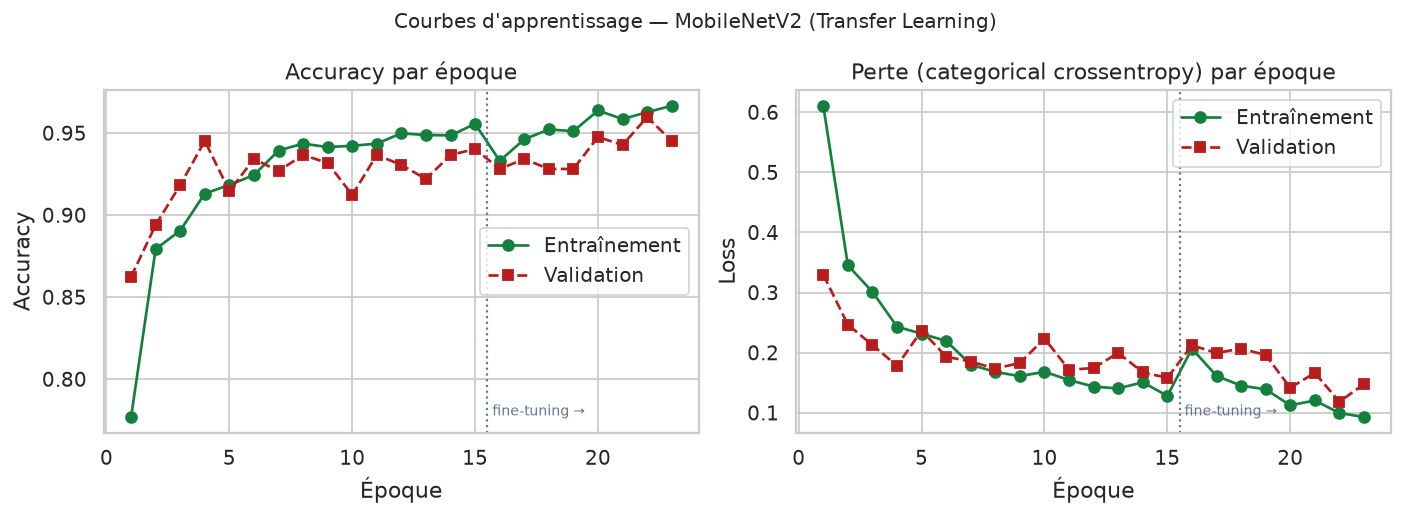
\includegraphics[width=0.68\linewidth,height=0.42\textheight,keepaspectratio]{../../../results/figures/training_curves.png}
\par\smallskip{\small\itshape Figure 5 --- Courbes d'apprentissage : accuracy et perte, entraînement et validation,}
\end{figure}

avec la séparation entre phase 1 et fine-tuning (ligne pointillée).*

L'accuracy d'entraînement progresse régulièrement de 77,7 \% à 96,7 \%. L'accuracy de validation atteint rapidement 94,5 \%, puis le fine-tuning permet de franchir la barre des 95 \% à l'époque 22 (\textbf{95,98 \%}). La perte de validation descend de 0,33 à 0,12. L'écart final entre entraînement (96,7 \%) et validation (95,98 \%) reste modéré, ce qui indique un sur-apprentissage limité.

\subsection{Métriques globales sur le test}

\begin{center}\small\itshape Tableau 12 --- Métriques globales du modèle sur l'ensemble de test.\end{center}
{\footnotesize
\begin{longtable}{@{}>{\raggedright\arraybackslash}p{0.28\linewidth}>{\raggedright\arraybackslash}p{0.58\linewidth}@{}}
\toprule
\textbf{Métrique} & \textbf{Valeur} \\
\midrule
\endhead
\bottomrule
\endlastfoot
Accuracy & \textbf{95,85 \%} \\
Precision (macro) & 95,47 \% \\
Recall (macro) & 95,25 \% \\
F1-score (macro) & \textbf{95,34 \%} \\
Precision (pondérée) & 95,83 \% \\
Recall (pondéré) & 95,85 \% \\
F1-score (pondéré) & 95,82 \% \\
Images de test & 820 \\
Images mal classées & 34 (4,15 \%) \\
\end{longtable}
}

L'accuracy de 95,85 \% signifie que 786 images sur 820 ont été correctement classées. La faible différence entre les moyennes macro (95,34 \%) et pondérée (95,82 \%) indique que les performances sont relativement homogènes entre classes : le modèle n'a pas sacrifié les classes minoritaires au profit des classes majoritaires.

\subsection{Performances par classe}

\begin{center}\small\itshape Tableau 13 --- Métriques détaillées par classe.\end{center}
{\footnotesize
\begin{longtable}{@{}>{\raggedright\arraybackslash}p{0.18\linewidth}>{\raggedright\arraybackslash}p{0.14\linewidth}>{\raggedright\arraybackslash}p{0.14\linewidth}>{\raggedright\arraybackslash}p{0.14\linewidth}>{\raggedright\arraybackslash}p{0.14\linewidth}>{\raggedright\arraybackslash}p{0.14\linewidth}@{}}
\toprule
\textbf{Classe} & \textbf{Precision} & \textbf{Recall} & \textbf{F1-score} & \textbf{Support} & \textbf{Bien classées} \\
\midrule
\endhead
\bottomrule
\endlastfoot
Alternariose précoce & 93,66 \% & 88,67 \% & 91,10 \% & 150 & 133 \\
Mildiou de la tomate & 96,15 \% & 95,82 \% & 95,99 \% & 287 & 275 \\
Moisissure des feuilles & 94,52 \% & 96,50 \% & 95,50 \% & 143 & 138 \\
Feuille saine & 97,56 \% & 100,00 \% & 98,77 \% & 240 & 240 \\
\textbf{Macro} & \textbf{95,47 \%} & \textbf{95,25 \%} & \textbf{95,34 \%} & 820 & 786 \\
\end{longtable}
}

\begin{figure}[H]
\centering
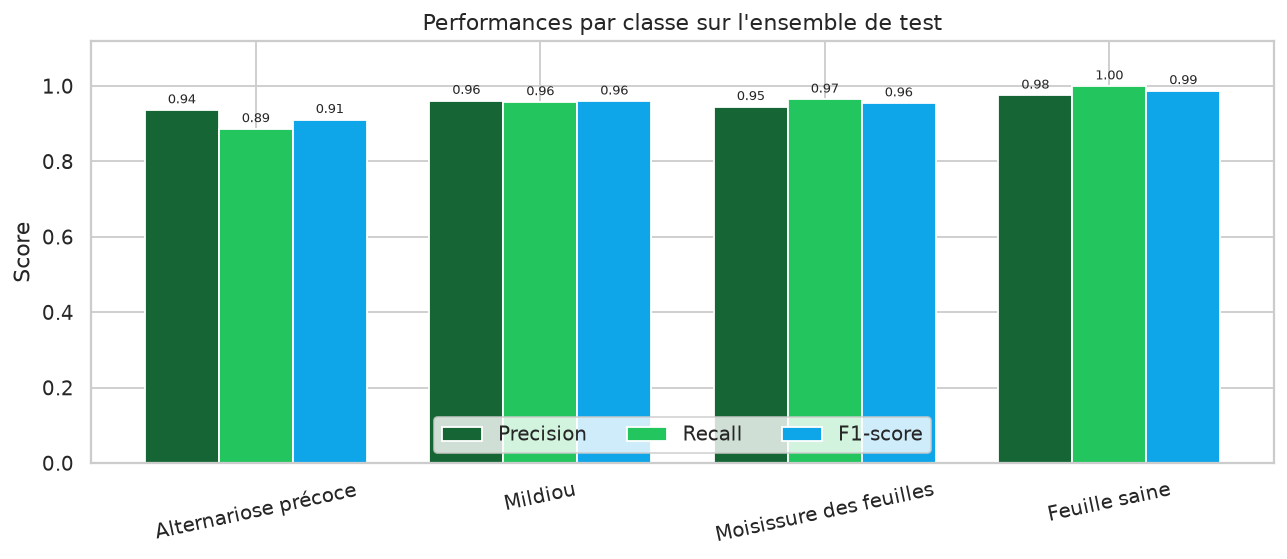
\includegraphics[width=0.68\linewidth,height=0.42\textheight,keepaspectratio]{../../../results/figures/per_class_performance.png}
\par\smallskip{\small\itshape Figure 6 --- Precision, recall et F1-score pour chacune des quatre classes.}
\end{figure}

Trois observations se dégagent :

\begin{enumerate}
\item \textbf{La classe \guillemotleft{} feuille saine \guillemotright{} est parfaitement détectée} (rappel de 100 \%). Aucune feuille saine n'a été classée comme malade, ce qui est le comportement souhaité pour un outil d'alerte : pas de fausse alerte sur un feuillage sain.
\item \textbf{L'alternariose précoce est la classe la plus difficile} (F1 = 91,10 \%, rappel de 88,67 \%) : 17 feuilles sur 150 lui échappent, dont 9 classées comme mildiou. Ces deux maladies produisent des taches brunes et leur ressemblance visuelle est bien connue en agronomie.
\item \textbf{Le mildiou et la moisissure} obtiennent des scores élevés (F1 $\approx$ 96 \%), cohérents avec leurs signatures visuelles plus marquées (lésions humides, duvet olive).
\end{enumerate}

\subsection{Matrice de confusion}

\begin{center}\small\itshape Tableau 14 --- Matrice de confusion (effectifs) sur les 820 images de test.\end{center}
{\footnotesize
\begin{longtable}{@{}>{\raggedright\arraybackslash}p{0.22\linewidth}>{\raggedright\arraybackslash}p{0.16\linewidth}>{\raggedright\arraybackslash}p{0.16\linewidth}>{\raggedright\arraybackslash}p{0.16\linewidth}>{\raggedright\arraybackslash}p{0.16\linewidth}@{}}
\toprule
\textbf{Réel \textbackslash{} Prédit} & \textbf{Alternariose} & \textbf{Mildiou} & \textbf{Moisissure} & \textbf{Saine} \\
\midrule
\endhead
\bottomrule
\endlastfoot
\textbf{Alternariose} & \textbf{133} & 9 & 4 & 4 \\
\textbf{Mildiou} & 6 & \textbf{275} & 4 & 2 \\
\textbf{Moisissure} & 3 & 2 & \textbf{138} & 0 \\
\textbf{Saine} & 0 & 0 & 0 & \textbf{240} \\
\end{longtable}
}

\begin{figure}[H]
\centering
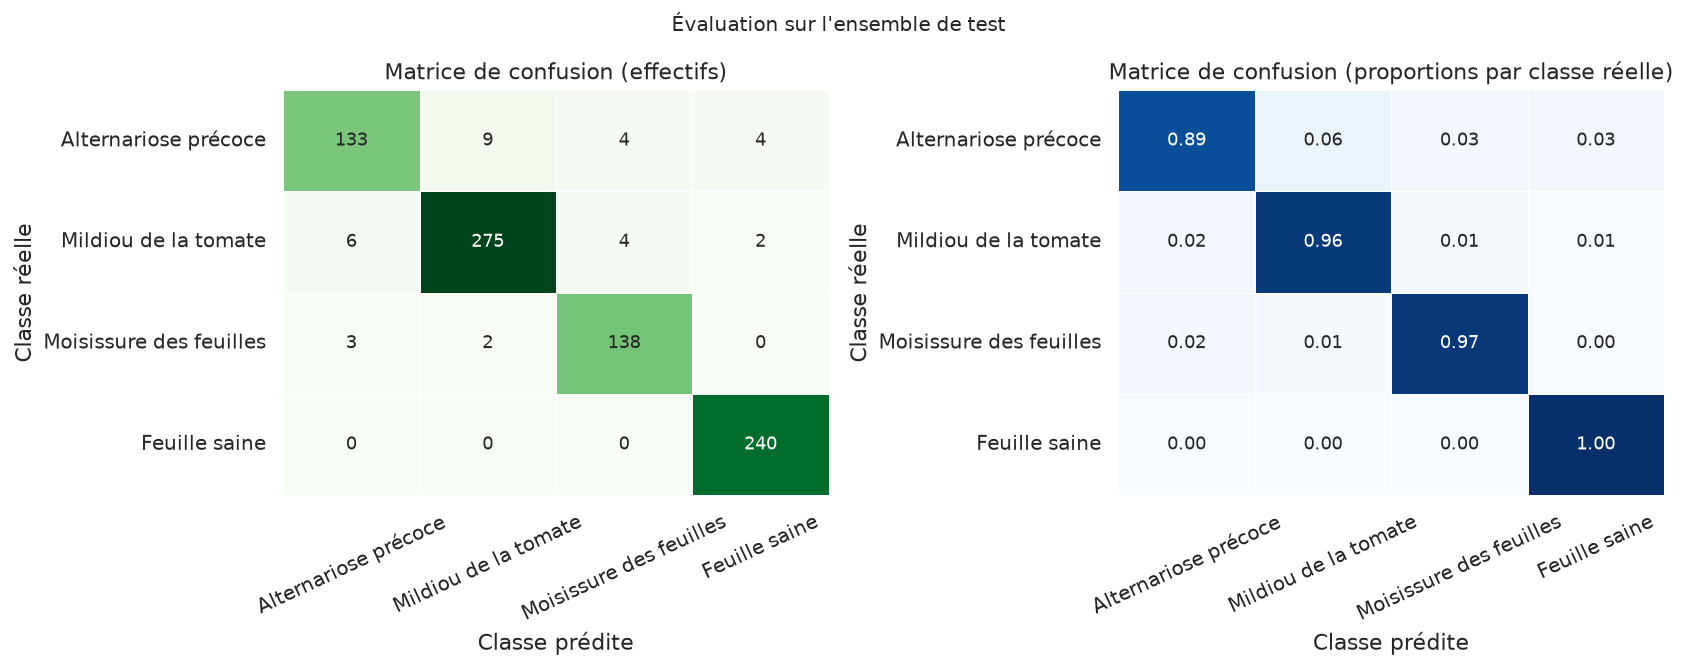
\includegraphics[width=0.68\linewidth,height=0.42\textheight,keepaspectratio]{../../../results/figures/confusion_matrix.png}
\par\smallskip{\small\itshape Figure 7 --- Matrice de confusion en effectifs (à gauche) et en proportions par classe}
\end{figure}

réelle (à droite).*

La lecture par ligne est la plus instructive : 88,7 \% des alternarioses sont correctement identifiées, 95,8 \% des mildious, 96,5 \% des moisissures et 100 \% des feuilles saines. La diagonale est nettement dominante, ce qui traduit un modèle globalement fiable. Les erreurs se concentrent sur la frontière alternariose / mildiou, avec 15 confusions croisées (9 + 6), soit près de la moitié des 34 erreurs totales.

\subsection{Analyse des erreurs}

\begin{center}\small\itshape Tableau 15 --- Statistiques de confiance et principales confusions.\end{center}
{\footnotesize
\begin{longtable}{@{}>{\raggedright\arraybackslash}p{0.28\linewidth}>{\raggedright\arraybackslash}p{0.58\linewidth}@{}}
\toprule
\textbf{Indicateur} & \textbf{Valeur} \\
\midrule
\endhead
\bottomrule
\endlastfoot
Erreurs totales & 34 / 820 (4,15 \%) \\
Confiance moyenne sur les prédictions correctes & 97,52 \% \\
Confiance moyenne sur les erreurs & 70,23 \% \\
Confiance médiane globale & 99,95 \% \\
Confusion la plus fréquente & Alternariose $\rightarrow$ Mildiou (9 cas) \\
\end{longtable}
}

La confiance moyenne des erreurs (70,2 \%) est très inférieure à celle des prédictions correctes (97,5 \%) : le modèle \guillemotleft{} sait \guillemotright{} en partie qu'il hésite. C'est un signal utile pour l'utilisateur et un argument en faveur de l'affichage de la distribution complète des probabilités plutôt que d'une classe unique.

\begin{figure}[H]
\centering
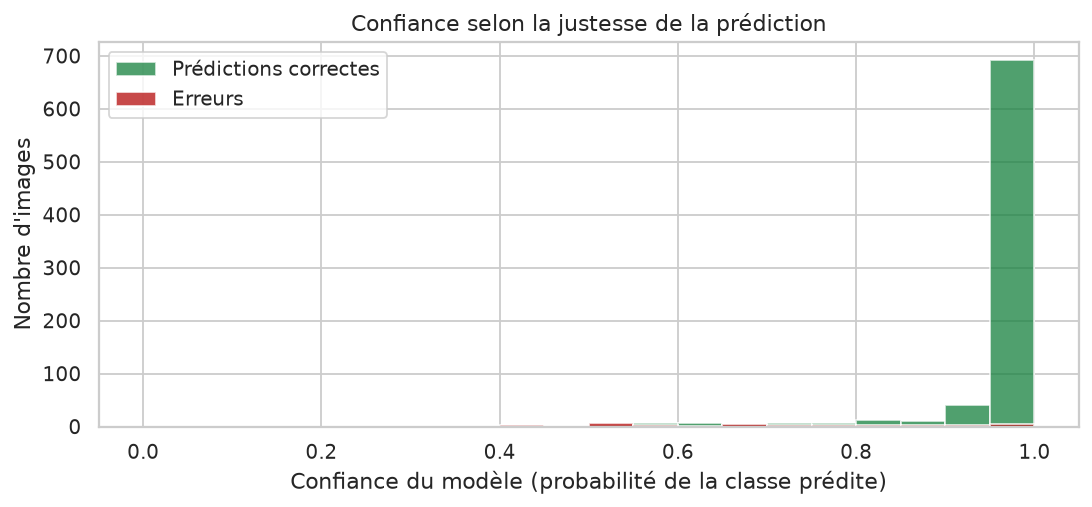
\includegraphics[width=0.68\linewidth,height=0.42\textheight,keepaspectratio]{../../../results/figures/confidence_distribution.png}
\par\smallskip{\small\itshape Figure 8 --- Distribution de la confiance selon que la prédiction est correcte ou non.}
\end{figure}

\begin{figure}[H]
\centering
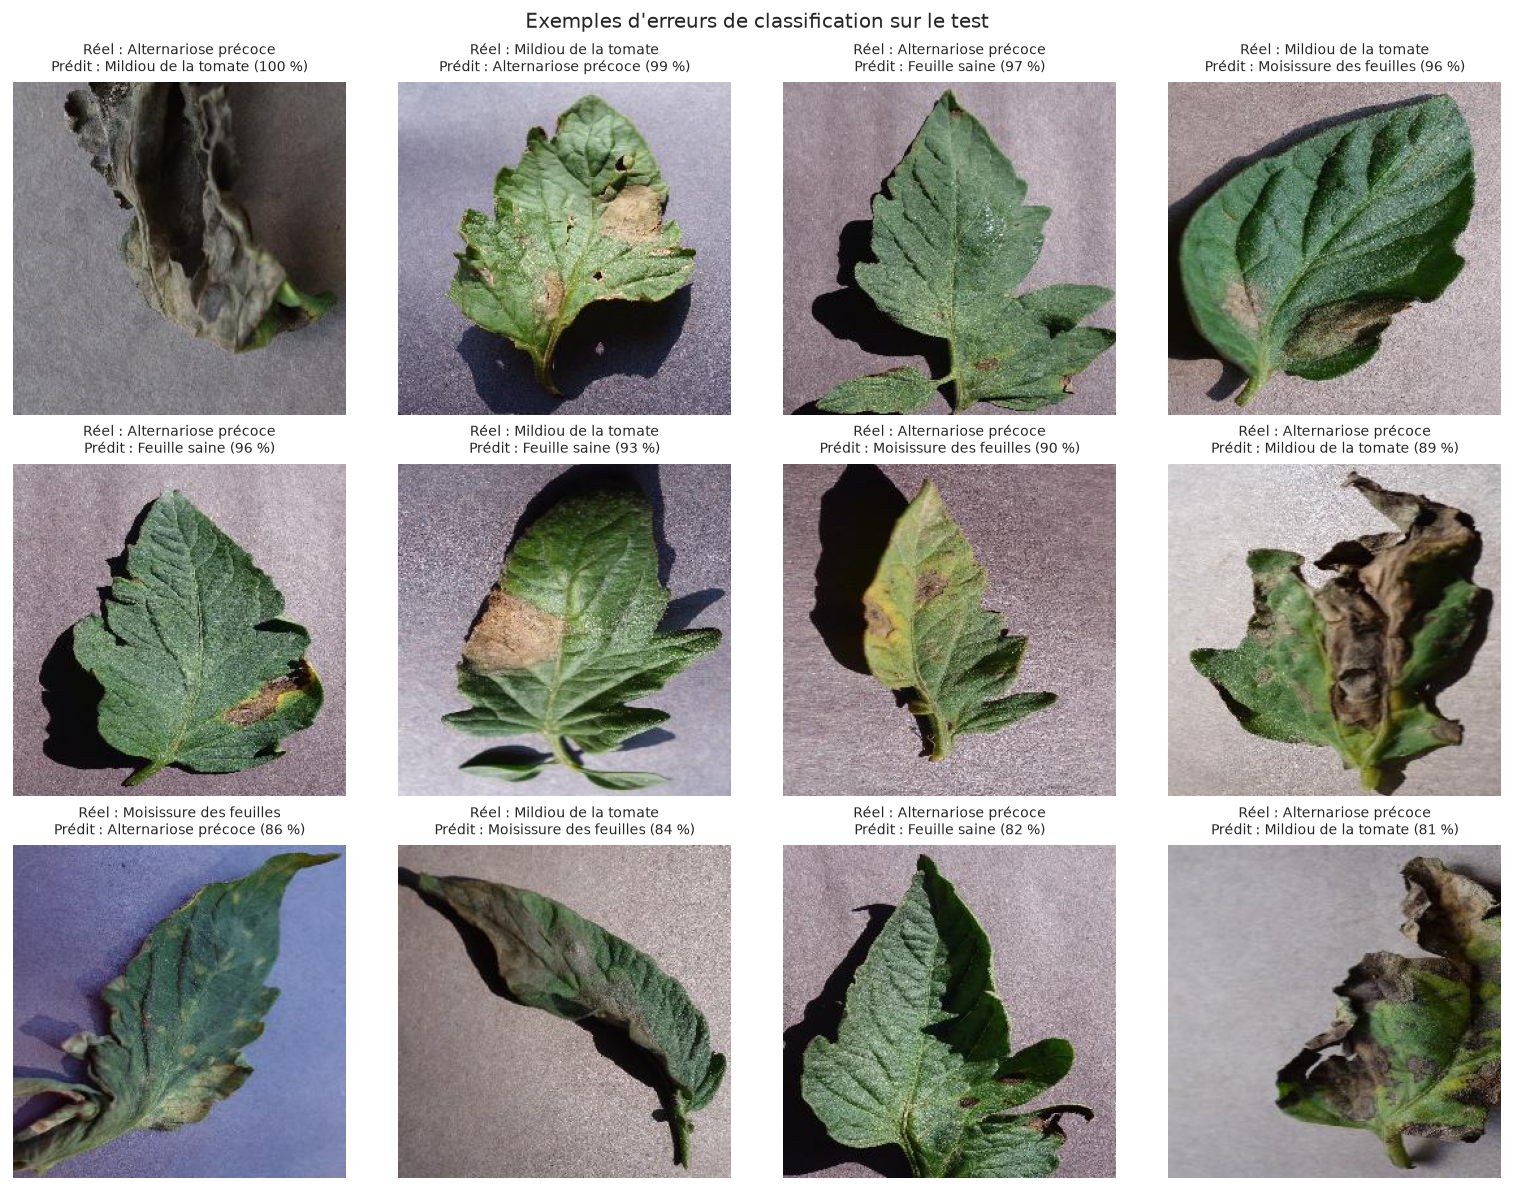
\includegraphics[width=0.68\linewidth,height=0.42\textheight,keepaspectratio]{../../../results/predictions/error_grid.png}
\par\smallskip{\small\itshape Figure 9 --- Exemples d'images mal classées : classe réelle, classe prédite et confiance.}
\end{figure}

La planche d'erreurs montre que les images mal classées sont souvent des cas ambigus : lésions peu contrastées, feuille partiellement floue, ou symptômes mélangés. Certaines images annotées \guillemotleft{} alternariose précoce \guillemotright{} présentent des taches sombres étendues qui évoquent visuellement le mildiou. Ces erreurs ne relèvent donc pas uniquement d'une faiblesse du modèle, mais aussi de la frontière floue entre deux pathologies.

\subsection{Temps d'inférence}

\begin{center}\small\itshape Tableau 16 --- Temps d'inférence mesurés sur le processeur de test.\end{center}
{\footnotesize
\begin{longtable}{@{}>{\raggedright\arraybackslash}p{0.28\linewidth}>{\raggedright\arraybackslash}p{0.58\linewidth}@{}}
\toprule
\textbf{Contexte} & \textbf{Durée observée} \\
\midrule
\endhead
\bottomrule
\endlastfoot
Première requête (chargement + échauffement) & $\approx$ 880 ms \\
Requêtes suivantes (modèle en mémoire) & 68 -- 80 ms \\
Batch d'évaluation (16 images) & $\approx$ 1,2 s, soit $\approx$ 75 ms par image \\
\end{longtable}
}

Le chargement unique du modèle au démarrage permet de répondre en moins de 100 ms par image, ce qui rend l'expérience fluide dans le navigateur. La première requête est plus lente en raison de l'initialisation des graphes TensorFlow.

\section{Évaluation et interprétation des métriques}
\label{sec:13}% Évaluation et interprétation des métriques

\subsection{Lecture critique de l'accuracy}

Une accuracy de 95,85 \% sur un jeu de test indépendant est un résultat solide pour un projet réalisé sans GPU et avec un budget d'époques réduit. Il faut néanmoins rappeler qu'un tel chiffre n'a de sens que replacé dans son contexte :

\begin{itemize}
\item le test provient de la \textbf{même distribution} que l'entraînement (même dataset, même protocole de prise de vue), ce qui facilite la tâche ;
\item la classe majoritaire représente 35 \% du test ; un classifieur naïf atteindrait déjà environ 35 \% d'accuracy, et un modèle prédisant toujours \guillemotleft{} mildiou \guillemotright{} obtiendrait 35 \% ;
\item les 820 images de test sont peu nombreuses à l'échelle des variations possibles d'une feuille de tomate malade.
\end{itemize}

L'accuracy est donc un indicateur de faisabilité, pas une garantie de performance sur le terrain.

\subsection{Cohérence entre les métriques}

Les quatre métriques macro sont comprises entre 95,25 \% et 95,47 \%, avec un F1 de 95,34 \%. Cette homogénéité signifie que le modèle n'est pas seulement bon sur les classes majoritaires : il conserve un bon rappel sur la moisissure (143 images seulement) et sur l'alternariose (150 images). Les poids de classes et la Data Augmentation ont probablement contribué à cet équilibre.

La precision (95,47 \%) est légèrement supérieure au recall (95,25 \%) : le modèle commet un peu plus de faux négatifs que de faux positifs. Dans un contexte de détection de maladie, ce compromis est discutable : manquer une feuille malade (faux négatif) peut être plus coûteux que signaler à tort une feuille saine. Un ajustement du seuil de décision, ou une pondération plus forte des classes malades, pourrait être envisagé.

\subsection{Interprétation des confusions}

Les confusions observées sont \textbf{biologiquement cohérentes} :

\begin{itemize}
\item \textbf{alternariose $\rightarrow$ mildiou (9 cas)} : les deux maladies produisent des taches brunes irrégulières ; à un stade avancé, l'alternariose perd ses anneaux concentriques et ressemble au mildiou ;
\item \textbf{mildiou $\rightarrow$ alternariose (6 cas)} : symétrique du cas précédent, souvent sur des lésions jeunes ou des images peu contrastées ;
\item \textbf{alternariose $\rightarrow$ feuille saine (4 cas)} : taches rares ou très petites, insuffisantes pour déclencher la classe malade ;
\item \textbf{mildiou $\rightarrow$ moisissure (4 cas)} et \textbf{alternariose $\rightarrow$ moisissure (4 cas)} : images présentant des plages jaunies communes aux deux pathologies.
\end{itemize}

Aucune confusion n'implique la classe \guillemotleft{} feuille saine \guillemotright{} en sortie : le modèle ne prend jamais une feuille malade pour une feuille saine de manière significative (2 cas de mildiou classés sains au maximum). C'est un point rassurant pour un usage d'alerte.

\subsection{Calibration et sur-confiance}

La confiance médiane (99,95 \%) est très élevée, et 100 \% des feuilles saines du test sont prédites avec une confiance proche de 1. Les réseaux de neurones modernes sont connus pour être \textbf{mal calibrés} : leurs probabilités softmax sont souvent trop tranchées. Un score de 100 \% ne signifie donc pas une certitude absolue, mais une forte activation du modèle.

L'écart de confiance entre prédictions correctes (97,5 \%) et erreurs (70,2 \%) montre que la confiance reste informative. Une perspective d'amélioration serait d'appliquer une \textbf{température scaling} ou une calibration de Platt sur l'ensemble de validation, afin de produire des probabilités plus réalistes.

\subsection{Positionnement par rapport à la littérature}

Mohanty et al. (2016) rapportent des accuracies supérieures à 99 \% sur PlantVillage avec des architectures comme AlexNet et GoogLeNet, sur l'ensemble des 38 classes et avec un protocole d'entraînement bien plus long. Nos 95,85 \% sur 4 classes ne sont pas directement comparables : le périmètre est plus restreint, le budget d'entraînement beaucoup plus faible (23 époques, CPU) et le découpage différent. Le résultat confirme néanmoins la tendance de fond de la littérature : sur PlantVillage, les CNN pré-entraînés atteignent une précision élevée avec un effort d'entraînement modéré.

\section{Discussion des résultats}
\label{sec:14}% Discussion des résultats

\subsection{Apport du Transfer Learning}

La progression observée valide l'intérêt du Transfer Learning :

\begin{center}\small\itshape Tableau 17 --- Progression de la validation au fil de l'expérience.\end{center}
{\footnotesize
\begin{longtable}{@{}>{\raggedright\arraybackslash}p{0.28\linewidth}>{\raggedright\arraybackslash}p{0.58\linewidth}@{}}
\toprule
\textbf{Étape} & \textbf{Accuracy de validation} \\
\midrule
\endhead
\bottomrule
\endlastfoot
Époque 1 (base gelée) & 86,24 \% \\
Meilleure phase 1 (époque 4) & 94,52 \% \\
Meilleure phase 2 (époque 22) & \textbf{95,98 \%} \\
\end{longtable}
}

Atteindre 86 \% dès la première époque, avec seulement 164 484 paramètres entraînables, aurait été impossible avec un réseau initialisé aléatoirement. Le gain du fine-tuning (+1,46 point) est plus modeste mais réel : il montre que les filtres profonds de MobileNetV2, initialement spécialisés sur ImageNet, bénéficient d'un ajustement aux textures de feuilles.

\subsection{Variabilité et sensibilité aux hyperparamètres}

La courbe de validation est irrégulière (oscillations de $\pm$2 points entre époques voisines). Trois facteurs expliquent cette variabilité :

\begin{enumerate}
\item la taille limitée du jeu de validation (821 images, soit environ 26 lots de 32) ;
\item l'application aléatoire de la Data Augmentation, qui modifie la difficulté des lots ;
\item le déséquilibre des classes, partiellement compensé par les poids de classes.
\end{enumerate}

Un usage plus stable serait obtenu avec une validation croisée à k plis, plus coûteuse en temps de calcul mais beaucoup plus robuste pour estimer la performance réelle.

\subsection{Coût de calcul et pertinence de MobileNetV2}

Le modèle complet ne pèse que 2,4 millions de paramètres et environ 24 Mo sur disque. Une époque d'entraînement dure 90 secondes sur deux cœurs, et une prédiction 70 ms. Ces chiffres confirment que MobileNetV2 est un choix adapté à un déploiement local, sur un ordinateur portable ou un mini-serveur, sans GPU ni service cloud. Un modèle plus profond (ResNet-50, EfficientNet-B3) aurait probablement apporté quelques points supplémentaires mais au prix d'un temps d'entraînement multiplié par 5 à 10 dans notre environnement.

\subsection{Qualité des données versus complexité du modèle}

Le principal facteur limitant n'est pas la capacité du modèle mais la \textbf{nature des données}. Les images PlantVillage sont prises en laboratoire, sur fond uniforme, avec une feuille unique et un éclairage contrôlé. Sur des photographies de terrain (feuillage dense, arrière-plan complexe, ombres, reflets, flou de bougé), les performances chuteraient très probablement. Améliorer le dataset (images de terrain, plusieurs feuilles par image, conditions variées) serait plus rentable que complexifier l'architecture.

\subsection{Enseignements méthodologiques}

Ce projet illustre plusieurs principes importants :

\begin{itemize}
\item \textbf{l'identité du prétraitement} entre entraînement et inférence est critique : elle est ici garantie par un module unique et vérifiée par un test ;
\item \textbf{la prévention des fuites} (doublons, split) conditionne la validité des métriques ;
\item \textbf{le suivi de la validation} (Early Stopping, checkpoint) évite de conserver un modèle dégradé : sans \texttt{initial\_\allowbreak{}value\_\allowbreak{}threshold}, le modèle final aurait été moins bon que celui de la phase 1 ;
\item \textbf{l'analyse des erreurs} apporte plus d'information que l'accuracy globale : elle révèle les frontières ambiguës entre maladies.
\end{itemize}

\section{Limites et perspectives d'amélioration}
\label{sec:15}% Limites et perspectives d'amélioration

\subsection{Limites du système actuel}

\textbf{Limites liées aux données}

\begin{itemize}
\item quatre classes seulement, alors que PlantVillage en compte 38 et que la tomate connaît une dizaine de maladies foliaires courantes ;
\item images de laboratoire, non représentatives des conditions de terrain ;
\item déséquilibre entre classes (952 à 1 909 images) ;
\item absence de regroupement par feuille (\emph{leaf grouping}), qui peut laisser passer des quasi-doublons entre ensembles ;
\item jeu de test de 820 images, insuffisant pour une estimation à $\pm$0,5 point près.
\end{itemize}

\textbf{Limites liées au modèle}

\begin{itemize}
\item une seule architecture et un seul protocole testés, faute de temps de calcul ;
\item pas de validation croisée ;
\item probabilités mal calibrées (sur-confiance) ;
\item pas d'explicabilité intégrée : l'utilisateur ne voit pas quelles zones de la feuille ont motivé la décision ;
\item pas de détection d'image hors domaine (une photo de fleur serait classée dans une des quatre catégories).
\end{itemize}

\textbf{Limites liées à l'application}

\begin{itemize}
\item pas de déploiement en production : serveur de développement Flask, sans HTTPS ;
\item une seule image analysée à la fois, sans traitement par lot dans l'interface ;
\item pas d'historique ni de suivi des analyses : choix de simplicité, aucune donnée n'est conservée ;
\item interface en français uniquement.
\end{itemize}

\subsection{Perspectives techniques}

\begin{enumerate}
\item \textbf{Explicabilité (Grad-CAM)} : produire une carte de chaleur des zones discriminantes, superposée à l'image, afin de renforcer la confiance de l'utilisateur et de détecter les décisions fondées sur des artefacts.
\item \textbf{Détection d'inconnu} : ajouter un seuil de rejet ou une classe \guillemotleft{} autre \guillemotright{} entraînée sur des images hors domaine, pour éviter de classer n'importe quelle image.
\item \textbf{Calibration des probabilités} : température scaling sur l'ensemble de validation.
\item \textbf{Validation croisée} à 5 plis pour une estimation plus fiable des performances.
\item \textbf{Comparaison d'architectures} : MobileNetV3, EfficientNet-B0, ResNet-50, avec le même protocole, pour objectiver le compromis précision / coût.
\item \textbf{Quantification et export} : conversion du modèle en TensorFlow Lite (INT8) ou ONNX pour un déploiement mobile.
\item \textbf{Augmentation plus agressive et adaptée} : mélange d'images (\emph{MixUp}, \emph{CutMix}), simulation d'ombres et de fonds variés, pour préparer le passage au terrain.
\item \textbf{Suivi d'expériences} : intégration de MLflow ou de TensorBoard pour comparer systématiquement les runs.
\end{enumerate}

\subsection{Perspectives applicatives}

\begin{itemize}
\item prise de photo directe depuis le smartphone (API \texttt{getUserMedia}) ;
\item export PDF d'une fiche de résultat ;
\item mode hors-ligne complet avec un modèle quantifié exécuté dans le navigateur (TensorFlow.js) ;
\item extension à d'autres cultures (pomme de terre, vigne, pommier) ;
\item interface multilingue.
\end{itemize}

\section{Éthique et impacts du système}
\label{sec:16}% Éthique et impacts du système

Un système de vision artificielle appliqué à l'agriculture ne soulève pas seulement des questions techniques. Parce qu'il produit une recommandation qu'un utilisateur pourrait suivre pour traiter une culture, il engage une responsabilité : celle de dire clairement ce qu'il fait, ce qu'il ne fait pas, et avec quelles données il a été construit. Cette section explicite le cadre d'usage, les risques identifiés et les mesures prises ou recommandées pour les atténuer.

\subsection{Usage prévu et limites de responsabilité}

L'usage prévu est \textbf{pédagogique et expérimental} : illustrer une chaîne complète de Deep Learning, de la donnée brute à l'application. Le système n'est ni un dispositif médical ni un outil de diagnostic agricole certifié. Trois précautions sont appliquées :

\begin{itemize}
\item un avertissement explicite figure dans le README et dans l'interface (page \guillemotleft{} À propos \guillemotright{}) ;
\item l'application affiche \textbf{les quatre probabilités}, et non une classe unique, afin que l'utilisateur voie l'incertitude du modèle ;
\item aucune prescription de traitement (dose, produit, fréquence) n'est proposée : les fiches maladies décrivent des symptômes et des principes de prévention, pas une ordonnance.
\end{itemize}

Toute décision de traitement doit rester celle d'un agronome ou d'un technicien, sur la base d'une observation de terrain. Le modèle ne qualifie ni la gravité ni le stade de l'infection, deux informations déterminantes pour décider d'une intervention.

\subsection{Données : licence, représentativité et biais}

\textbf{Licence et redistribution.} Le dépôt PlantVillage ne comporte pas de fichier de licence explicite. Les images sont donc utilisées dans un cadre strictement académique, ne sont \textbf{pas redistribuées} et ne sont pas versionnées dans le dépôt Git (\texttt{.gitignore}), ce qui respecte la source et évite toute réutilisation non contrôlée.

\textbf{Biais de représentativité.} Le jeu de données est constitué de feuilles isolées, photographiées en laboratoire sur fond uniforme, dans des conditions contrôlées et pour un nombre limité de variétés. Il sous-représente les situations réelles : symptômes précoces ou atypiques, attaques multiples, feuilles sales ou flétries, arrière-plans végétaux, éclairages rasants, photos de smartphone compressées. Le modèle n'a jamais vu ces conditions : \textbf{aucune mesure de performance hors domaine n'est disponible}, et rien ne permet d'affirmer que les 95,85 \% obtenus se transposeraient au champ. Ce biais est le plus important du projet et il est explicité dans les limites (\S{}15.1).

\textbf{Biais hérité du pré-entraînement.} Les poids ImageNet proviennent d'images web, avec leurs propres déséquilibres géographiques et culturels. Le transfer learning accélère l'apprentissage mais transmet une partie de ces biais, impossible à quantifier ici.

\textbf{Déséquilibre entre classes.} Les effectifs vont de 952 à 1 909 images. Les poids de classes compensent partiellement ce déséquilibre à l'entraînement, mais la classe la plus petite (moisissure, 143 images de test) reste celle dont l'estimation est la plus fragile, avec un intervalle de confiance plus large.

\textbf{Données personnelles dans le dataset.} Les images ne contiennent pas de données personnelles identifiantes à notre connaissance, mais leurs métadonnées EXIF n'ont pas fait l'objet d'un audit exhaustif ; ce point est signalé par prudence.

\subsection{Vie privée des utilisateurs de l'application}

Le principe appliqué est la \textbf{minimisation absolue} : l'image téléversée n'est \textbf{jamais écrite sur le disque}. Elle est décodée en mémoire, convertie en tenseur, passée au modèle, puis oubliée à la fin de la requête. L'application ne conserve donc ni image, ni nom de fichier, ni résultat : aucune analyse n'est consultable après coup, aucune donnée personnelle n'est stockée.

Mesures techniques concrètes :

\begin{itemize}
\item \textbf{traitement en mémoire} : le flux du fichier est lu directement par Pillow, sans écriture dans un répertoire temporaire ;
\item \textbf{aucun chemin construit} à partir du nom fourni par le client : ce nom sert uniquement à vérifier l'extension, ce qui exclut toute traversée de répertoire ;
\item \textbf{aucun envoi à un tiers} : l'inférence est exécutée par le serveur local, sans API externe ni service cloud ;
\item \textbf{aucun cookie de suivi, aucun compte, aucune adresse IP enregistrée} : l'application ne tient pas de session et n'a pas de base de données.
\end{itemize}

Limites assumées : le serveur de développement Flask sert la page \textbf{en HTTP}, sans chiffrement ; une image transite donc en clair sur le réseau si l'application est exposée autre part qu'en local, et les journaux du serveur conservent l'heure et le code de réponse des requêtes. Pour un déploiement réel, il faudrait ajouter HTTPS, une politique de rétention des journaux et une information explicite des utilisateurs. Ces points sont documentés comme limites et non masqués.

\subsection{Risque d'un mauvais diagnostic}

Sur 820 images, 34 erreurs (4,15 \%) subsistent. Leur concentration est le point sensible : 15 confusions croisées entre \textbf{alternariose précoce} et \textbf{mildiou}, deux maladies dont les lésions se ressemblent mais dont la gestion diffère. Une erreur dans ce couple peut conduire à un traitement inadapté, donc à une perte de récolte ou à un usage inutile de fongicides.

Deux risques symétriques doivent être nommés :

\begin{itemize}
\item \textbf{faux négatif} (maladie prédite saine) : risque de propagation silencieuse, le plus grave agronomiquement ; la classe saine est toutefois celle qui obtient le meilleur rappel (100 \% sur le test), ce qui limite ce risque dans le domaine étudié ;
\item \textbf{faux positif} (sain prédit malade) : traitement inutile, coût économique et intrants supplémentaires.
\end{itemize}

La confiance moyenne des erreurs (70,23 \%) est nettement inférieure à celle des prédictions correctes (97,52 \%), mais elle reste élevée pour certaines erreurs : l'affichage de la confiance \textbf{ne suffit pas} à lui seul à alerter l'utilisateur. C'est pourquoi un seuil de rejet et une carte d'attention (Grad-CAM) figurent parmi les perspectives prioritaires.

\subsection{Équité et accessibilité}

Le choix de MobileNetV2 (2,4 millions de paramètres, inférence d'environ 70 ms sur CPU) relève aussi d'un souci d'équité d'accès : le système fonctionne sans GPU et sur un poste modeste, condition indispensable pour un usage dans de petites exploitations. Le modèle est en outre suffisamment compact pour envisager une exécution embarquée après quantification.

À l'inverse, trois barrières subsistent : l'interface est uniquement en français ; elle suppose un smartphone ou un ordinateur et une instance accessible ; et \textbf{aucune mesure de performance par sous-groupe} (type d'appareil, conditions d'éclairage, variété, stade de la maladie) n'a été réalisée. Il n'est donc pas possible d'affirmer que le modèle est équitable entre ces situations : c'est un audit à conduire avant tout usage réel.

\subsection{Impact environnemental et coût de calcul}

L'entraînement complet a duré \textbf{37,7 minutes de CPU} (23,4 min pour la phase 1, 14,3 min pour le fine-tuning) sur un processeur à deux cœurs, sans GPU. Le transfer learning est ici le principal levier environnemental : il évite d'entraîner un CNN from scratch, qui exigerait plusieurs heures à plusieurs jours de calcul pour un résultat souvent inférieur. L'inférence (environ 70 ms par image) est négligeable à l'échelle d'un usage interactif.

Le projet ne fournit pas d'estimation en kWh ni en équivalent CO\textsubscript{2} : une telle estimation n'aurait de sens qu'avec la consommation réelle mesurée de la machine. Les recommandations associées sont de réutiliser le modèle existant plutôt que de réentraîner sans nécessité, et de privilégier la quantification pour l'inférence mobile.

\subsection{Conduite scientifique}

Toutes les valeurs du rapport proviennent d'un entraînement et d'une évaluation réellement exécutés ; aucune métrique n'est simulée ni recopiée d'une publication. Les figures et la fiche expérimentale sont générées par script à partir des fichiers de résultats, ce qui réduit le risque d'erreur de recopie. Le dataset n'est pas versionné, mais les scripts, les métriques, les prédictions et le modèle le sont, ce qui rend l'expérience auditable.

Deux réserves d'honnêteté accompagneront la lecture des chiffres : l'expérience repose sur \textbf{un seul run} (pas de validation croisée, donc pas d'estimation de la variabilité), et le budget d'époques a été réduit (15 + 8 au lieu de 30 + 15) faute de GPU. Les 95,85 \% ne doivent donc pas être présentés comme une borne supérieure de performance.

\subsection{Synthèse des risques et des mesures}

\begin{center}\small\itshape Tableau 18 --- Synthèse des risques éthiques identifiés et des mesures d'atténuation.\end{center}
{\footnotesize
\begin{longtable}{@{}>{\raggedright\arraybackslash}p{0.24\linewidth}>{\raggedright\arraybackslash}p{0.13\linewidth}>{\raggedright\arraybackslash}p{0.27\linewidth}>{\raggedright\arraybackslash}p{0.22\linewidth}@{}}
\toprule
\textbf{Risque} & \textbf{Gravité} & \textbf{Mesure en place} & \textbf{Mesure recommandée} \\
\midrule
\endhead
\bottomrule
\endlastfoot
Mauvais diagnostic suivi d'un traitement & Élevée & Avertissement explicite, 4 probabilités affichées, aucune prescription & Seuil de rejet, Grad-CAM, validation par un agronome \\
Écart entre laboratoire et terrain & Élevée & Limite documentée (\S{}15.1), pas de promesse de performance terrain & Constituer un jeu de test de terrain et le publier \\
Atteinte à la vie privée & Faible & Aucune image ni résultat conservé, traitement en mémoire, aucun compte & HTTPS et politique de journaux en cas de déploiement \\
Biais de représentation et d'équité & Moyenne & Déséquilibre traité par poids de classes, biais explicités & Audit par sous-groupe, augmentation de données variées \\
Inégalité d'accès à l'outil & Moyenne & Modèle léger, exécution CPU, aucune API payante & Interface multilingue, mode hors-ligne quantifié \\
Coût de calcul & Faible & Transfer learning, 37,7 min de CPU, pas de GPU & Réutiliser le modèle, quantifier pour l'inférence \\
\end{longtable}
}

En résumé, le projet ne revendique pas la neutralité : il rend explicites ses données, ses biais, ses erreurs et son domaine de validité, et il refuse de transformer une prédiction probabiliste en prescription agricole. Cette transparence est la condition minimale d'un usage responsable, et la première des améliorations à venir.

\section{Conclusion générale}
\label{sec:17}% Conclusion générale

Ce projet avait pour objectif de concevoir un système complet de détection et de classification des maladies de la feuille de tomate, depuis la donnée brute jusqu'à une application Web utilisable. Cet objectif a été atteint : un modèle MobileNetV2 adapté par Transfer Learning a été entraîné sur 3 811 images, évalué sur 820 images indépendantes, et intégré dans une application Flask en français.

Les résultats expérimentaux sont les suivants :

\begin{itemize}
\item \textbf{accuracy de 95,85 \%} sur l'ensemble de test ;
\item \textbf{F1-score macro de 95,34 \%}, avec des performances homogènes entre les quatre classes (de 91,10 \% à 98,77 \%) ;
\item \textbf{34 erreurs sur 820 images}, concentrées sur la frontière entre alternariose précoce et mildiou, deux maladies visuellement proches ;
\item \textbf{temps d'inférence d'environ 70 ms} par image, compatible avec une utilisation interactive ;
\item un modèle compact de \textbf{2,4 millions de paramètres}, entraînable et exécutable sans GPU.
\end{itemize}

Au-delà des chiffres, le projet apporte plusieurs contributions méthodologiques : un découpage rigoureux sans fuite de données, un prétraitement strictement identique entre entraînement et inférence (vérifié par un test), une évaluation complète avec matrice de confusion et analyse d'erreurs, une application sécurisée et testée, et une documentation qui distingue clairement ce qui a été mesuré de ce qui reste hypothétique.

Le système ne constitue pas un diagnostic agricole. Il s'agit d'un outil expérimental d'aide à la reconnaissance visuelle, dont les limites sont explicites : quatre classes, images de laboratoire, absence d'explicabilité et de détection d'inconnu. Les perspectives identifiées --- Grad-CAM, calibration, validation croisée, données de terrain, quantification --- tracent un chemin réaliste vers un outil plus robuste et réellement utilisable sur le terrain.

Sur le plan pédagogique, ce projet a permis de mettre en pratique l'ensemble de la chaîne d'un projet de Deep Learning : préparation et audit des données, choix d'architecture, Transfer Learning, régularisation, évaluation critique, intégration applicative, tests et documentation. Il illustre une idée essentielle : la performance d'un modèle dépend moins de sa complexité que de la qualité des données, de la rigueur du protocole et de l'honnêteté de l'interprétation.

\section{Références bibliographiques}
\label{sec:18}% Références bibliographiques

\begin{enumerate}
\item Hughes, D. P., \& Salathé, M. (2015). \emph{An open access repository of images on plant health to enable the development of mobile disease diagnostics}. arXiv:1511.08060.
\item Mohanty, S. P., Hughes, D. P., \& Salathé, M. (2016). Using deep learning for image-based plant disease detection. \emph{Frontiers in Plant Science}, 7, 1419. https://doi.org/10.3389/fpls.2016.01419
\item Sandler, M., Howard, A., Zhu, M., Zhmoginov, A., \& Chen, L.-C. (2018). MobileNetV2: Inverted residuals and linear bottlenecks. \emph{Proceedings of the IEEE Conference on Computer Vision and Pattern Recognition (CVPR)}, 4510--4520.
\item Howard, A. G., Zhu, M., Chen, B., Kalenichenko, D., Wang, W., Weyand, T., Andreetto, M., \& Adam, H. (2017). \emph{MobileNets: Efficient convolutional neural networks for mobile vision applications}. arXiv:1704.04861.
\item LeCun, Y., Bengio, Y., \& Hinton, G. (2015). Deep learning. \emph{Nature}, 521(7553), 436--444.
\item LeCun, Y., Bottou, L., Bengio, Y., \& Haffner, P. (1998). Gradient-based learning applied to document recognition. \emph{Proceedings of the IEEE}, 86(11), 2278--2324.
\item Krizhevsky, A., Sutskever, I., \& Hinton, G. E. (2012). ImageNet classification with deep convolutional neural networks. \emph{Advances in Neural Information Processing Systems (NeurIPS)}, 25, 1097--1105.
\item He, K., Zhang, X., Ren, S., \& Sun, J. (2016). Deep residual learning for image recognition. \emph{Proceedings of the IEEE Conference on Computer Vision and Pattern Recognition (CVPR)}, 770--778.
\item Simonyan, K., \& Zisserman, A. (2015). \emph{Very deep convolutional networks for large-scale image recognition}. arXiv:1409.1556.
\item Szegedy, C., Liu, W., Jia, Y., Sermanet, P., Reed, S., Anguelov, D., Erhan, D., Vanhoucke, V., \& Rabinovich, A. (2015). Going deeper with convolutions. \emph{Proceedings of the IEEE Conference on Computer Vision and Pattern Recognition (CVPR)}, 1--9.
\item Pan, S. J., \& Yang, Q. (2010). A survey on transfer learning. \emph{IEEE Transactions on Knowledge and Data Engineering}, 22(10), 1345--1359.
\item Shorten, C., \& Khoshgoftaar, T. M. (2019). A survey on image data augmentation for deep learning. \emph{Journal of Big Data}, 6(1), 60.
\item Kingma, D. P., \& Ba, J. (2015). \emph{Adam: A method for stochastic optimization}. arXiv:1412.6980.
\item Rumelhart, D. E., Hinton, G. E., \& Williams, R. J. (1986). Learning representations by back-propagating errors. \emph{Nature}, 323(6088), 533--536.
\item Srivastava, N., Hinton, G., Krizhevsky, A., Sutskever, I., \& Salakhutdinov, R. (2014). Dropout: A simple way to prevent neural networks from overfitting. \emph{Journal of Machine Learning Research}, 15(1), 1929--1958.
\item Selvaraju, R. R., Cogswell, M., Das, A., Vedantam, R., Parikh, D., \& Batra, D. (2017). Grad-CAM: Visual explanations from deep networks via gradient-based localization. \emph{Proceedings of the IEEE International Conference on Computer Vision (ICCV)}, 618--626.
\item Chollet, F. (2021). \emph{Deep Learning with Python} (2\textsuperscript{e} édition). Manning Publications.
\item Abadi, M. et al. (2016). TensorFlow: A system for large-scale machine learning. \emph{12th USENIX Symposium on Operating Systems Design and Implementation (OSDI)}, 265--283.
\end{enumerate}

\clearpage

\section*{Annexe --- Ressources du projet}
\addcontentsline{toc}{section}{Annexe --- Ressources du projet}

{\footnotesize
\begin{longtable}{@{}>{\raggedright\arraybackslash}p{0.28\linewidth}>{\raggedright\arraybackslash}p{0.58\linewidth}@{}}
\toprule
\textbf{Ressource} & \textbf{Emplacement} \\
\midrule
\endhead
\bottomrule
\endlastfoot
Code source complet & dépôt Git du projet \\
Notebook d'expérimentation & \texttt{notebooks/\allowbreak{}plant\_\allowbreak{}disease\_\allowbreak{}training.ipynb} \\
Script de téléchargement du dataset & \texttt{training/\allowbreak{}download\_\allowbreak{}dataset.py} \\
Préparation et découpage & \texttt{training/\allowbreak{}prepare\_\allowbreak{}data.py} \\
Entraînement & \texttt{training/\allowbreak{}train.py} \\
Évaluation et figures & \texttt{training/\allowbreak{}evaluate.py} \\
Prédiction en ligne de commande & \texttt{training/\allowbreak{}predict.py} \\
Modèle entraîné & \texttt{models/\allowbreak{}best\_\allowbreak{}model.keras} \\
Configuration et comptages & \texttt{models/\allowbreak{}training\_\allowbreak{}config.json} \\
Métriques détaillées & \texttt{results/\allowbreak{}metrics/\allowbreak{}evaluation.json} \\
Rapport de classification & \texttt{results/\allowbreak{}metrics/\allowbreak{}classification\_\allowbreak{}report.txt} \\
Figures & \texttt{results/\allowbreak{}figures/\allowbreak{}} \\
Prédictions et erreurs & \texttt{results/\allowbreak{}predictions/\allowbreak{}} \\
Tests automatisés & \texttt{tests/\allowbreak{}} \\
\end{longtable}
}

\end{document}
